\documentclass[aspectratio=169]{beamer}

\usepackage{amsmath, amssymb, amsxtra, amsthm, amsfonts}
\usetheme{moloch}
\usecolortheme{beaver}
\setbeamertemplate{footline}
{
  \leavevmode%
  \hbox{%
    \begin{beamercolorbox}[wd=.5\paperwidth,ht=2.25ex,dp=1ex,center]{author in head/foot}%
      \usebeamerfont{author in head/foot}\insertsection
    \end{beamercolorbox}%
    \begin{beamercolorbox}[wd=.5\paperwidth,ht=2.25ex,dp=1ex,right]{date in head/foot}%
      \usebeamerfont{date in head/foot}\inserttitle\hspace*{2em}
      \insertframenumber{} / \inserttotalframenumber\hspace*{2ex}
    \end{beamercolorbox}}%
  \vskip0pt%
}
\makeatother

\usepackage[english]{babel}
\usefonttheme{serif}

\usepackage{mathtools}
\usepackage{graphicx}
\usepackage{bm}
\usepackage{color}
\usepackage[dvipsnames,table]{xcolor}
\usepackage{tikz}
\usepackage{stanli}
\usepackage{verbatim}
\usepackage{tikz}
\usetikzlibrary{shapes,calc,through,3d,patterns}
\usetikzlibrary{decorations.pathreplacing}
\usetikzlibrary{arrows.meta,calc,positioning}

\usepackage{pgfplots}
\usepackage{siunitx} % For formatting numbers
\usepackage{hyperref}
\hypersetup{colorlinks=true,linkcolor=darkred}
\usepackage{multicol}
\usepackage[absolute,overlay,]{textpos}
\usepackage{pgfplots}
\pgfplotsset{width=10cm,compat=1.9}
\usepackage{subcaption}
\usepackage{multirow}
\usepackage{bbding}
\usepackage{arydshln}
\usepackage{mathtools}
\usepackage{tcolorbox}
\usepackage{animate}

\textblockorigin{80mm}{45mm}


\newtheorem{thm}{Theorem}
\newtheorem{cor}[thm]{Corollary}
\newtheorem{prop}[thm]{Proposition}
\newtheorem{lem}[thm]{Lemma}
\theoremstyle{remark}
\newtheorem*{rem}{Remark}

%Block def
\definecolor{darkred}{rgb}{0.6,0,0}
\setbeamertemplate{blocks}[rounded][shadow=false]
\setbeamercolor{block title}{bg=darkred!15,fg=black}
\setbeamercolor{block body}{bg=darkred!5,fg=black}

\setbeamercolor{itemize item}{fg=darkred}
\setbeamercolor{itemize subitem}{fg=darkred}
\setbeamercolor{itemize subsubitem}{fg=darkred}
\setbeamercolor{enumerate item}{fg=darkred}
\setbeamercolor{button}{bg=gray!30,fg=darkred}

\setbeamertemplate{itemize item}[square]
\setbeamertemplate{itemize subitem}[circle]
\setbeamertemplate{itemize subsubitem}[triangle]
\setbeamertemplate{enumerate items}[circle]
\setbeamercolor{item projected}{bg=darkred}

\newcommand{\bolddelta}{\boldsymbol\delta}
\newcommand{\boldxi}{\boldsymbol\xi}
\DeclareMathOperator*{\A}{\text{\raisebox{-0.2cm}{\Huge A}}}




\title{Dynamic analysis of shells}
\subtitle{Special structural elements}
\author{ME473 Dynamic finite element analysis of structures}
\institute{Stefano Burzio}
\date{2025}

\begin{document}
\usenavigationsymbolstemplate{}
{\setbeamertemplate{footline}{}

  \frame{\titlepage
    \begin{tikzpicture}[overlay, remember picture]
      \node[anchor=north east, xshift=-.9cm] at (current page.north east) {
\includegraphics[width=2cm]{../images/epfl_logo.png}};
      \node[anchor=south east, xshift=-.87cm, yshift=.05cm] at (current page.south east)  {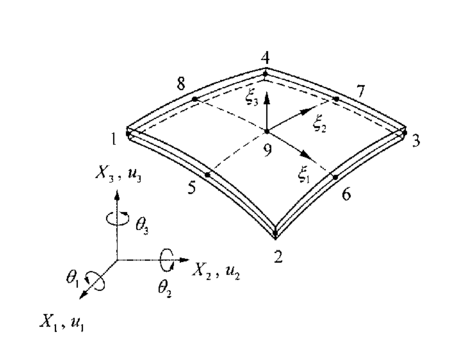
\includegraphics[height=3.5cm]{../images/shellElem.png}};
    \end{tikzpicture}
  }

  \begin{frame}{Where do we stand?}
    \begin{center}
      \begin{tabular}{|c|l|l|l|}
        \hline
        \rowcolor{darkred!20}\textbf{Week} & \textbf{Module}                                & \textbf{Lecture topic}             & \textbf{Mini-projects} \\
        \hline
        1                                  & \multirow{5}{7em}{Linear elastodynamics}       & Strong and weak forms              &                        \\ \cline{1-1} \cline{3-4}
        2                                  &                                                & Galerkin and FE methods            &                        \\ \cline{1-1} \cline{3-4}
        3                                  &                                                & Systematisation of the procedure   & Groups formation       \\ \cline{1-1} \cline{3-4}
        4                                  &                                                & 3d elements, numerical integration & Project 1 statement    \\
        \cline{1-1} \cline{3-4}
        \hline
        5                                  & \multirow{5}{7em}{Special structural elements} & Bars and trusses                   &                        \\
        \cline{1-1} \cline{3-4} 6          &                                                & Beams, frames and grids            &                        \\
        \cline{1-1} \cline{3-4} 7          &                                                & Kirchhoff-Love plates              &                        \\
        \cline{1-1} \cline{3-4}
        8                                  &                                                & Reissner-Mindlin plates            &                        \\
        \cline{1-1} \cline{3-4}
        9                                  &                                                & Shells                             & Project 1 submission   \\
        \hline
      \end{tabular}
    \end{center}
    \vspace{1cm}
  \end{frame}

  \begin{frame}
    \textbf{\large Summary}
    \begin{itemize}
      \item Recap week 8
      \item Thin shell elements
      \item Example: modal analysis of simply supported thin shell
    \end{itemize}
    \vspace{.5cm}

    \textbf{\large Recommended readings}
    \begin{itemize}
      \item[(N)] Neto et al., Engineering Computation of Structures (chap. 6.3)
      \item[(P)] Petyt, Introduction to finite element vibration analysis (chap. 8)
      \item[(O)] Ochsner, PDE for classical structural members (chap. 7)
      \item[(G)] Gmür, Méthode des éléments finis (chap. 3)
    \end{itemize}
  \end{frame}
}

\section{Recap week 8 \\ Vibrations of Reissner-Mindlin plates}
 {\setbeamercolor{background canvas}{bg=darkred!5}
  \setbeamercolor{block body}{bg=darkred!5,fg=black}
  \begin{frame}{Plates theories}
    \begin{columns}
      \begin{column}{0.5\textwidth}
        \textbf{Thin plates}
        \begin{center}
          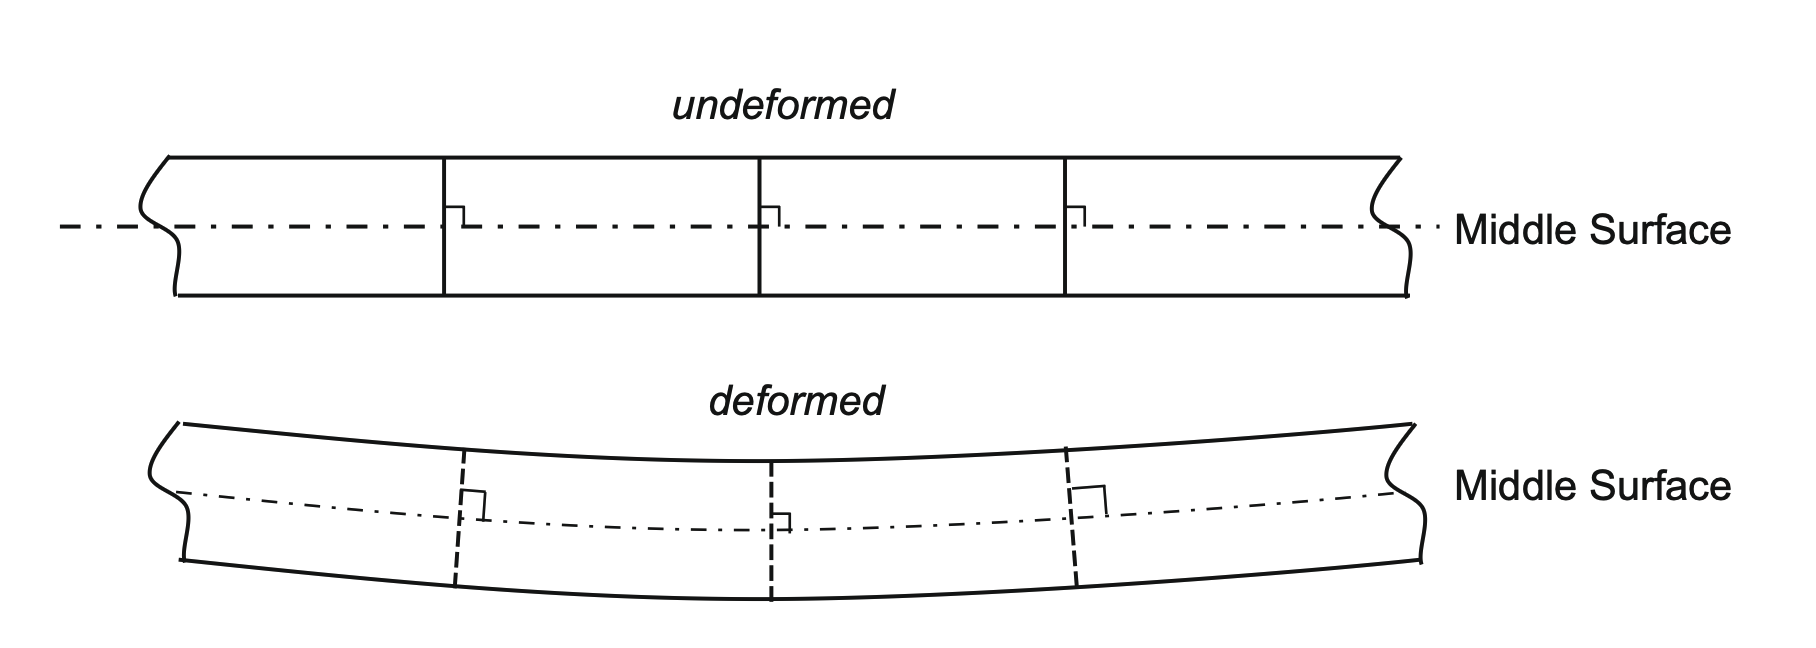
\includegraphics[width=6cm]{../images/KirchhoffPlateHp.png}
        \end{center}
        \begin{itemize}
          \item Planarity and orthogonality of the cross-sectional planes.
          \item Generalized displacements:
                \begin{block}{}
                  $$\mathbf u=\begin{bmatrix}
                      -z\partial_x u_3 &
                      -z\partial_y u_3 &
                      u_3
                    \end{bmatrix}^T$$
                \end{block}
        \end{itemize}
      \end{column}

      \begin{column}{0.5\textwidth}
        \textbf{Thick plates}
        \begin{center}
          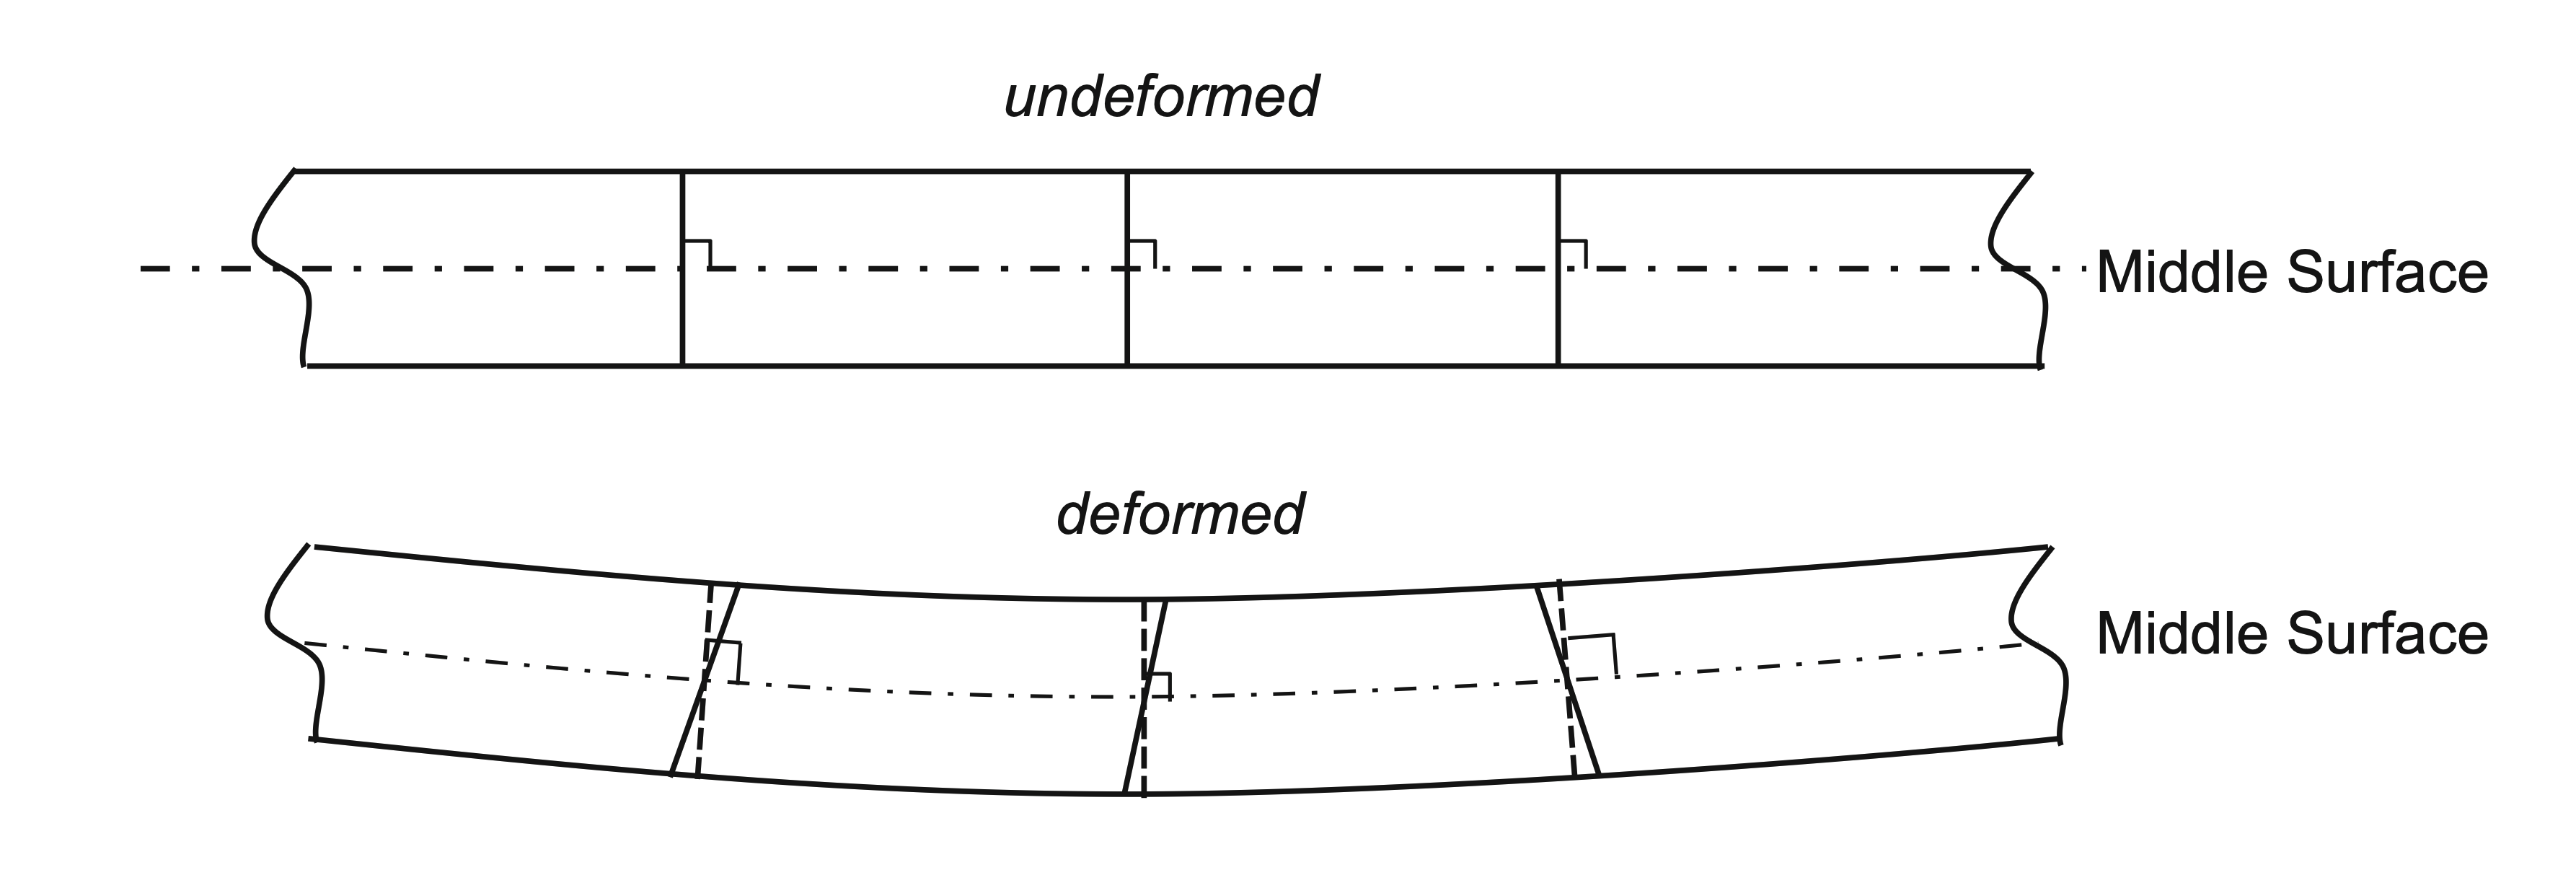
\includegraphics[width=6cm]{../images/ReissnerPlateHp.png}
        \end{center}
        \begin{itemize}
          \item Planarity of the cross-sectional planes.
          \item Generalized displacements:
                \begin{block}{}
                  $$\mathbf u=\begin{bmatrix}
                      z \phi_2  &
                      -z \phi_1 &
                      u_3
                    \end{bmatrix}^T$$
                \end{block}
        \end{itemize}
      \end{column}
    \end{columns}
  \end{frame}

  \begin{frame}{Strong form for Reissner-Mindlin plate bending}
    \begin{block}{}
      Let $\Omega=[-a,a]\times[-b,b]$ be a rectangular plate. Find the transverse displacement $u_{3}\in C^2(\Omega\times[0,T])$ and the rotations $\phi_1,\ \phi_2\in C^2(\Omega\times[0,T])$ such that
      $$
        \nabla_m^T \overline{\boldsymbol{C}}\nabla_r\mathbf{u}+\mathbf f=\mathbf{I} \ddot{\mathbf u} \qquad \text{  on  }\Omega\times]0,T[
      $$
      \vspace{-0.5cm}
      \begin{columns}
        \begin{column}{0.55\textwidth}
          \begin{itemize}
            \item boundary conditions (\emph{simply supported}):
                  \vspace{-0.2cm}
                  \[
                    \begin{aligned}
                       & u_3 = 0\qquad   & \text{in }\partial\Omega\times]0,T[   \\
                       & \phi_2 =0\qquad & \text{in }\partial\Omega_1\times]0,T[ \\
                       & \phi_1 =0\qquad & \text{in }\partial\Omega_2\times]0,T[
                    \end{aligned}
                  \]
            \item
                  initial conditions:
                  \vspace{-0.2cm}
                  \[
                    \begin{aligned}
                       & \color{orange}{\mathbf u(\cdot, 0) =  \mathbf u_0 \quad \text{in }\Omega}      \\
                       & \color{orange}{\dot{\mathbf u}(\cdot, 0) = \mathbf v_0 \quad \text{in }\Omega} \\
                    \end{aligned}
                  \]
          \end{itemize}
        \end{column}

        \begin{column}{0.38\textwidth}
          \begin{center}
            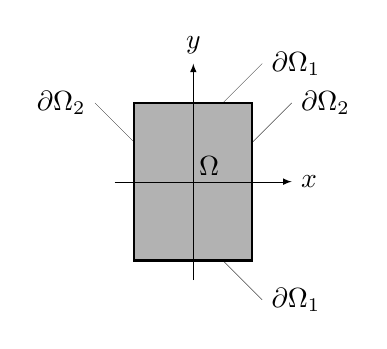
\begin{tikzpicture}[scale=0.5]
              \def\a{3}
              \def\b{4}
              % Draw the rectangle
              \filldraw[fill=gray!60, draw=black,thick] (0,0) rectangle (\a,\b);
              %axis
              \draw[-latex,ultra thin] (-0.5,\b/2) -- (\a+1,\b/2) node[right]{$x$};
              \draw[-latex, ultra thin] (\a/2,-0.5) -- (\a/2,\b+1)node[above]{$y$};
              % Omega
              \node at (\a/2+0.4,\b/2+0.4) {$\Omega$};
              \draw[ultra thin] (3*\a/4,\b) -- (3*\a/4+1,\b+1) node[right]{$\partial\Omega_1$};
              \draw[ultra thin] (\a,3*\b/4) -- (\a+1,3*\b/4+1) node[right]{$\partial\Omega_2$};
              \draw[ultra thin] (3*\a/4,0) -- (3*\a/4+1,-1) node[right]{$\partial\Omega_1$};
              \draw[ultra thin] (0,3*\b/4) -- (-1,3*\b/4+1) node[left]{$\partial\Omega_2$};
            \end{tikzpicture}
          \end{center}
        \end{column}
      \end{columns}
    \end{block}
  \end{frame}

  \begin{frame}{Definitions}
    \begin{itemize}
      \item Reissner-Mindlin differential operators:
            {\small$$\nabla_r=\begin{bmatrix}
                \nabla_b \\ \nabla_s
              \end{bmatrix}=\begin{bmatrix}
                0          & 0           & \partial_x \\
                0          & -\partial_y & 0          \\
                0          & -\partial_x & \partial_y \\
                \partial_x & 0           & 1          \\
                \partial_y & -1          & 0          \\
              \end{bmatrix},\qquad\text{and}\qquad \nabla_m=\begin{bmatrix}
                \nabla_b \\ \nabla_s
              \end{bmatrix}=\begin{bmatrix}
                0          & 0           & \partial_x \\
                0          & -\partial_y & 0          \\
                0          & -\partial_x & \partial_y \\
                \partial_x & 0           & -1         \\
                \partial_y & 1           & 0          \\
              \end{bmatrix}.$$}
      \item Constitutive matrix for isotropic materials: {\small$\overline{\boldsymbol{C}}=\begin{bmatrix}\overline{\boldsymbol{C}_b} & \mathbf 0                   \\
               \mathbf 0                   & \overline{\boldsymbol{C}_s}
              \end{bmatrix}$}
            {\small$$ \overline{\boldsymbol{C}_b}=\frac{Eh^3}{12(1 - \nu^2)}\begin{bmatrix}
                1   & \nu & 0                 \\
                \nu & 1   & 0                 \\
                0   & 0   & \frac{1 - \nu}{2}
              \end{bmatrix}\qquad\text{and}\qquad \overline{\boldsymbol{C}_s}= \frac{Ekh}{2(1 + \nu)}\begin{bmatrix}
                1 & 0 \\
                0 & 1 \\
              \end{bmatrix}.$$}
      \item Mass moment of inertia matrix: {\small$\mathbf I=\begin{bmatrix}
                \rho h & 0           & 0           \\
                0      & \rho h^3/12 & 0           \\
                0      & 0           & \rho h^3/12 \\
              \end{bmatrix}$}.
    \end{itemize}
  \end{frame}

  \begin{frame}{Generalized displacements approximation}
    \begin{block}{}
      Since the rotations $\phi_1$ and $\phi_2$ are defined independently of the transversal displacement $u_3$, the discretization uses \textbf{bilinear Lagrangian finite elements}:
      \vspace{-0.3cm}
      \begin{align*}
        {}^e \mathbf u^{h}(\mathbf x,t) & ={}^e \mathbf H(\mathbf x){}^e\mathbf q(t) = \sum_{i=1}^{4}{}^eh_{i}(\mathbf x){}^e\mathbf q^{i}(t)
      \end{align*}
      \vspace{-0.5cm}
    \end{block}
    \begin{itemize}
      \item ${}^e\mathbf H(\mathbf x)$ is a $3\times 12$ matrix of \textbf{shape functions} ($\mathbf I$ is the $3\times 3$ identity matrix.):
            $$
              {}^e\mathbf H
              =\left[
                \begin{array}{c;{2pt/2pt}c;{2pt/2pt}c;{2pt/2pt}c}
                  h_{1}\mathbf I & h_{2}\mathbf I & h_{3}\mathbf I & h_{4}\mathbf I \\
                \end{array} \right] = \begin{bmatrix}
                {}^eh_1 & 0       & 0       &       & {}^eh_{4} & 0         & 0         \\
                0       & {}^eh_1 & 0       & \dots & 0         & {}^eh_{4} & 0         \\
                0       & 0       & {}^eh_1 &       & 0         & 0         & {}^eh_{4} \\
              \end{bmatrix}
            $$

      \item ${}^e\mathbf q^i(t)=\begin{bmatrix}
                {}^e d^{i}(t) \\ {}^e \theta^{i}_1(t) \\ {}^e \theta^{i}_2(t)
              \end{bmatrix}$ and ${}^e\mathbf u^h=\begin{bmatrix}
                {}^e u_3^h \\ {}^e \phi_1^h \\ {}^e \phi_2^h
              \end{bmatrix}$ are the generalized displacements of node $i$ and inside the element $e$ respectively.
    \end{itemize}
  \end{frame}

  \begin{frame}{Elementary matrices and loads vector}
    \begin{itemize}
      \item \textbf{Elementary stiffness matrix} ($12\times 12$):
            $$
              {}^e\mathbf K =\underbrace{\int_{{}^e\Omega}{}^e\mathbf B_b^T\overline{\boldsymbol{C}_b}{}^e\mathbf B_b\, d\Omega}_\text{${}^e\mathbf K_b$}+\underbrace{\int_{{}^e\Omega}{}^e\mathbf B_s^T\overline{\boldsymbol{C}_s}{}^e\mathbf B_s\, d\Omega}_\text{${}^e\mathbf K_s$}
            $$
            \vspace{-0.3cm}
            \begin{itemize}
              \item Bending strain-displacement matrix:
                    ${}^e\mathbf B_b=\nabla_b {}^e\mathbf H$.
              \item Shear strain-displacement matrix:
                    ${}^e\mathbf B_s=\nabla_s {}^e\mathbf H$.
                    \vspace{0.2cm}
            \end{itemize}
      \item \textbf{Elementary mass matrix} ($12\times 12$):
            $${}^e\mathbf M=\int_{{}^e\Omega}  {}^e\mathbf H^T\, \mathbf{I}\, {}^e\mathbf H \, d\Omega.$$
      \item \textbf{Elementary applied forces vector} ($12\times 1$):
            $${}^e\mathbf r(t)=\int_{{}^e\Omega} {}^e\mathbf H^{T}\mathbf f\, d\Omega.$$
    \end{itemize}
  \end{frame}

  \begin{frame}{Modal shapes for SSSS thick plates (span/thickness = 0.1)}
    \vspace{-0.1cm}
    \begin{figure}[h]
      \begin{subfigure}{0.48\textwidth}
        \centering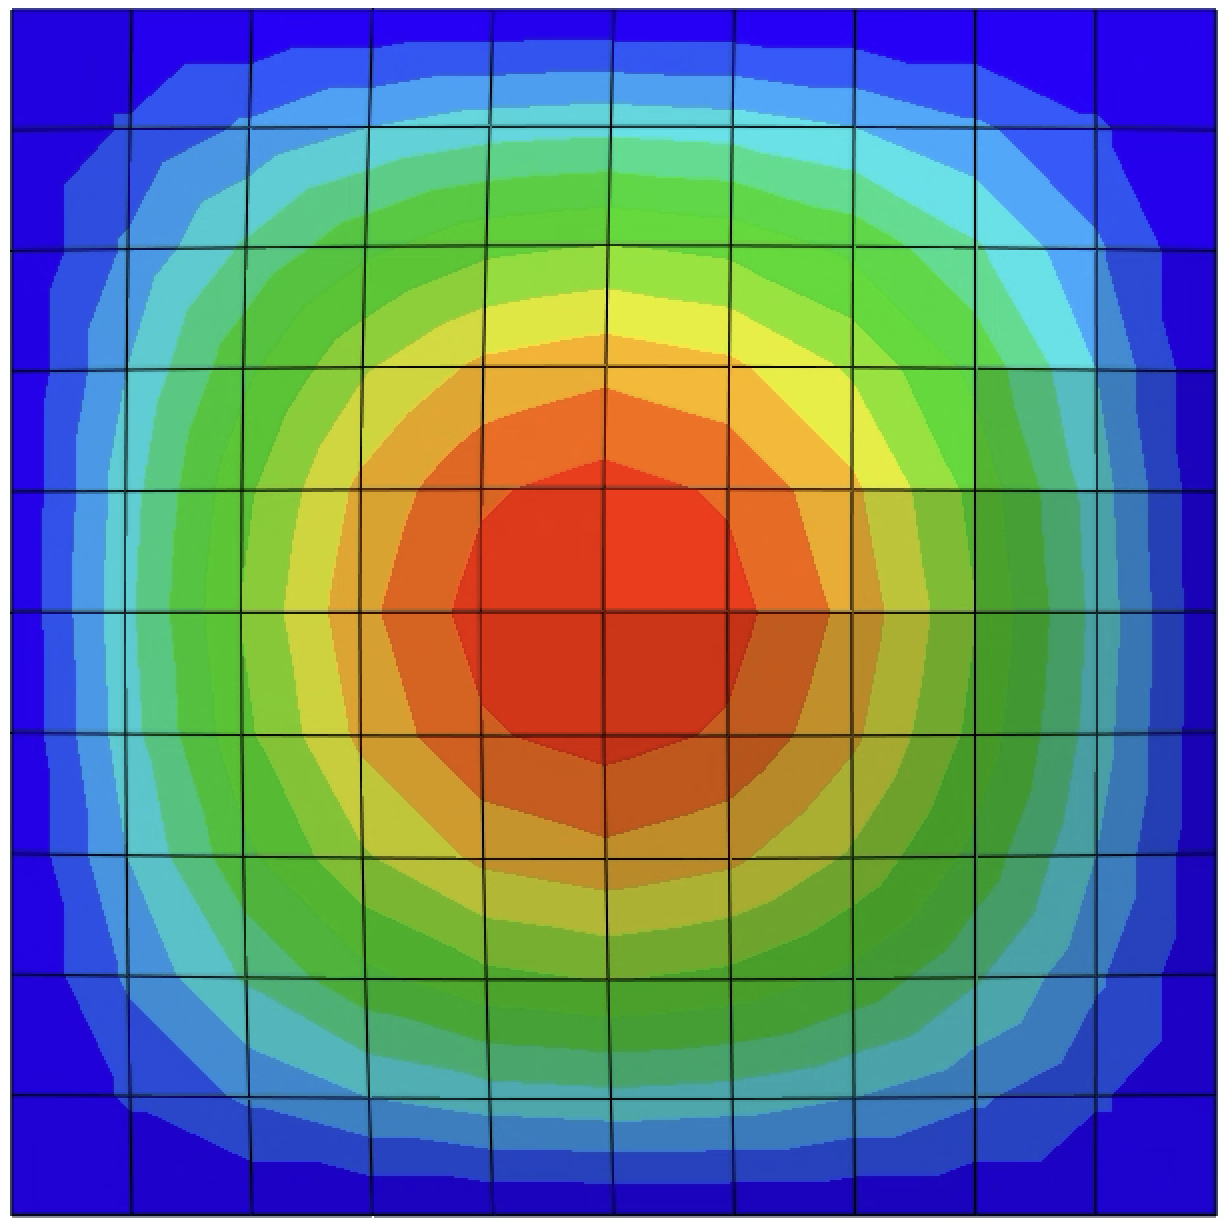
\includegraphics[width=3cm, height=3cm]{../images/thick1.png}
        \caption{Mode shape 1: $\omega_{11}^h=9.672$ Hz}
      \end{subfigure}
      \begin{subfigure}{0.48\textwidth}
        \centering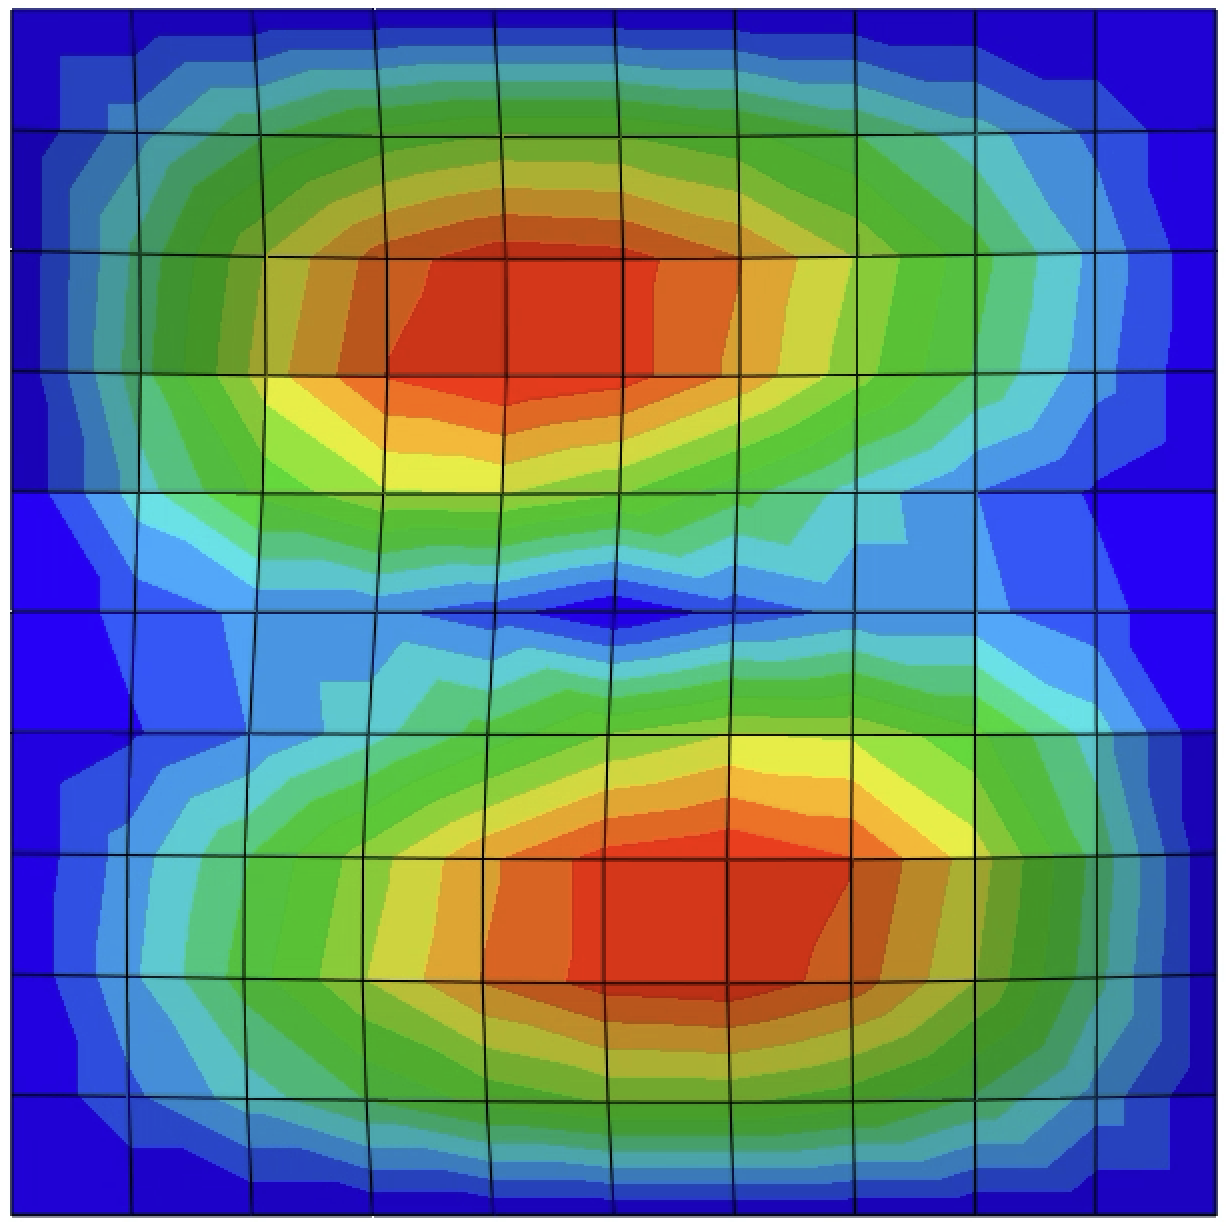
\includegraphics[width=3cm, height=3cm]{../images/thick2.png}
        \caption{Mode shape 2: $\omega_{12}^h=23.643$ Hz}
      \end{subfigure}
      \newline
      \begin{subfigure}{0.48\textwidth}
        \centering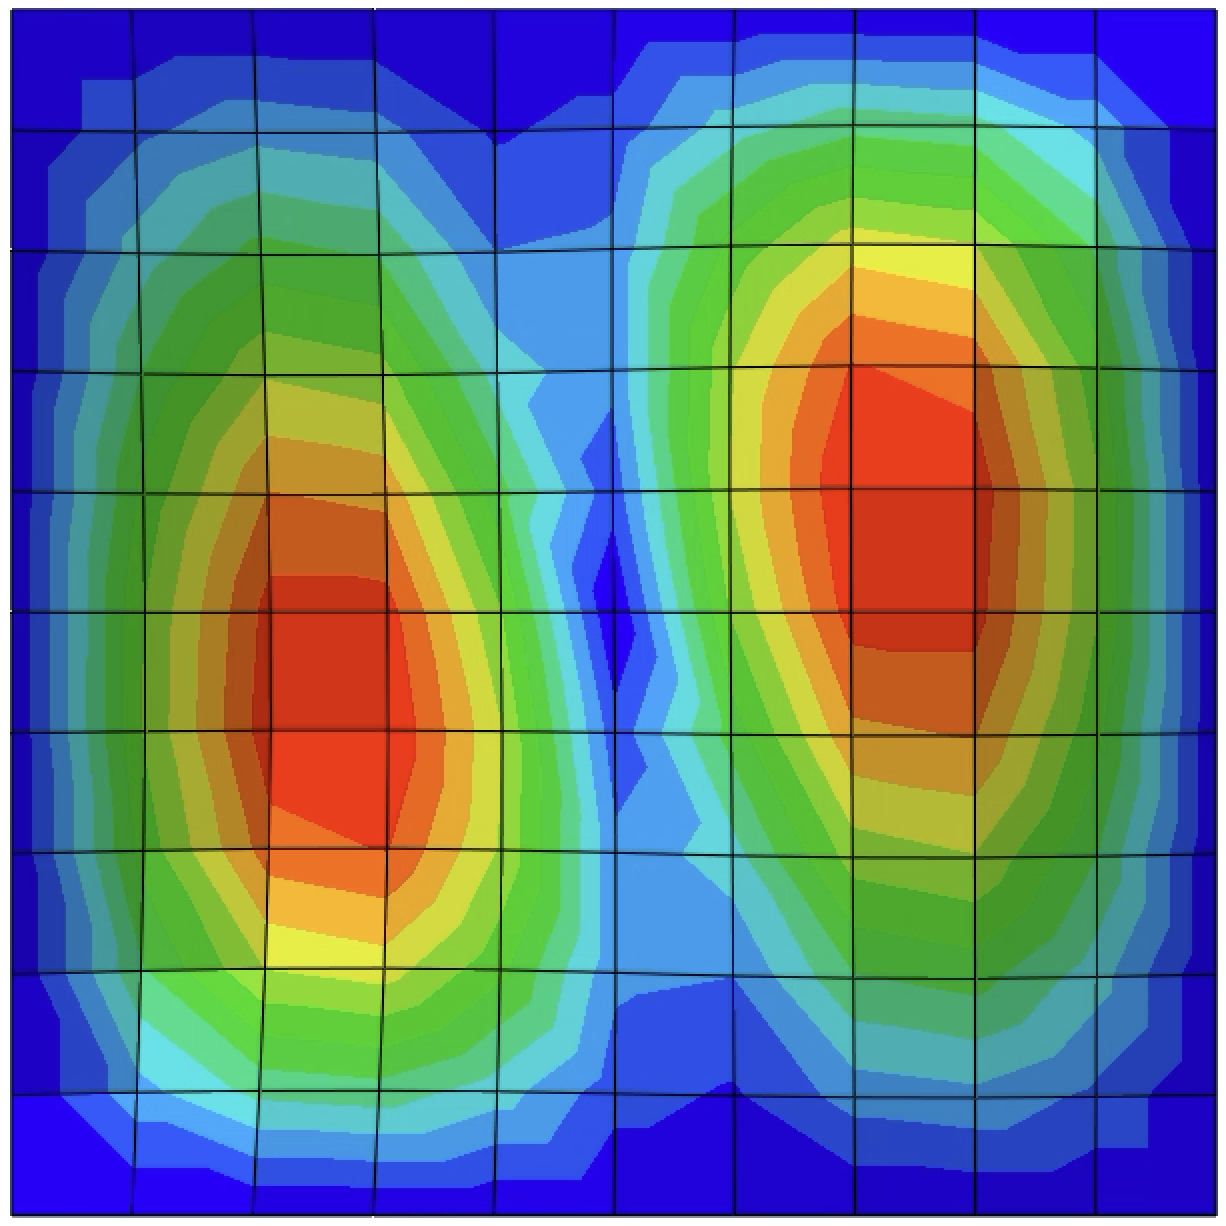
\includegraphics[width=3cm, height=3cm]{../images/thick3.png}
        \caption{Mode shape 3: $\omega_{21}^h=23.643$ Hz}
      \end{subfigure}
      \begin{subfigure}{0.48\textwidth}
        \centering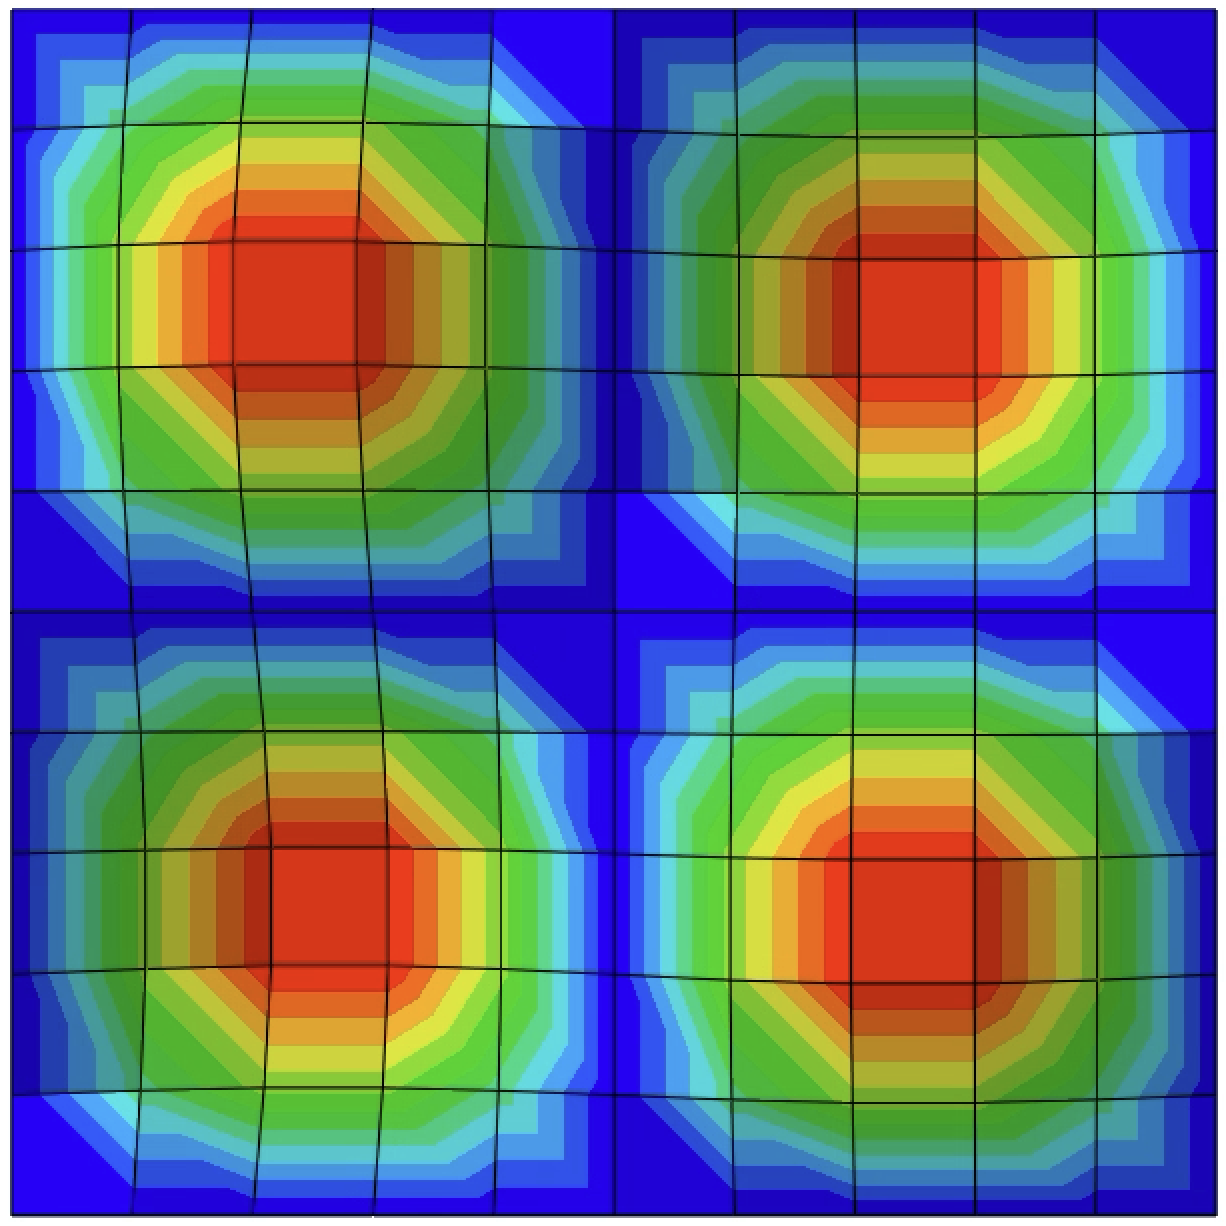
\includegraphics[width=3cm, height=3cm]{../images/thick4.png}
        \caption{Mode shape 4: $\omega_{22}^h=36.114$ Hz}
      \end{subfigure}
    \end{figure}
  \end{frame}

  \begin{frame}{Modal shapes for SSSS thin plates  (span/thickness = 0.01)}
    \vspace{-0.1cm}
    \begin{figure}[h]
      \begin{subfigure}{0.48\textwidth}
        \centering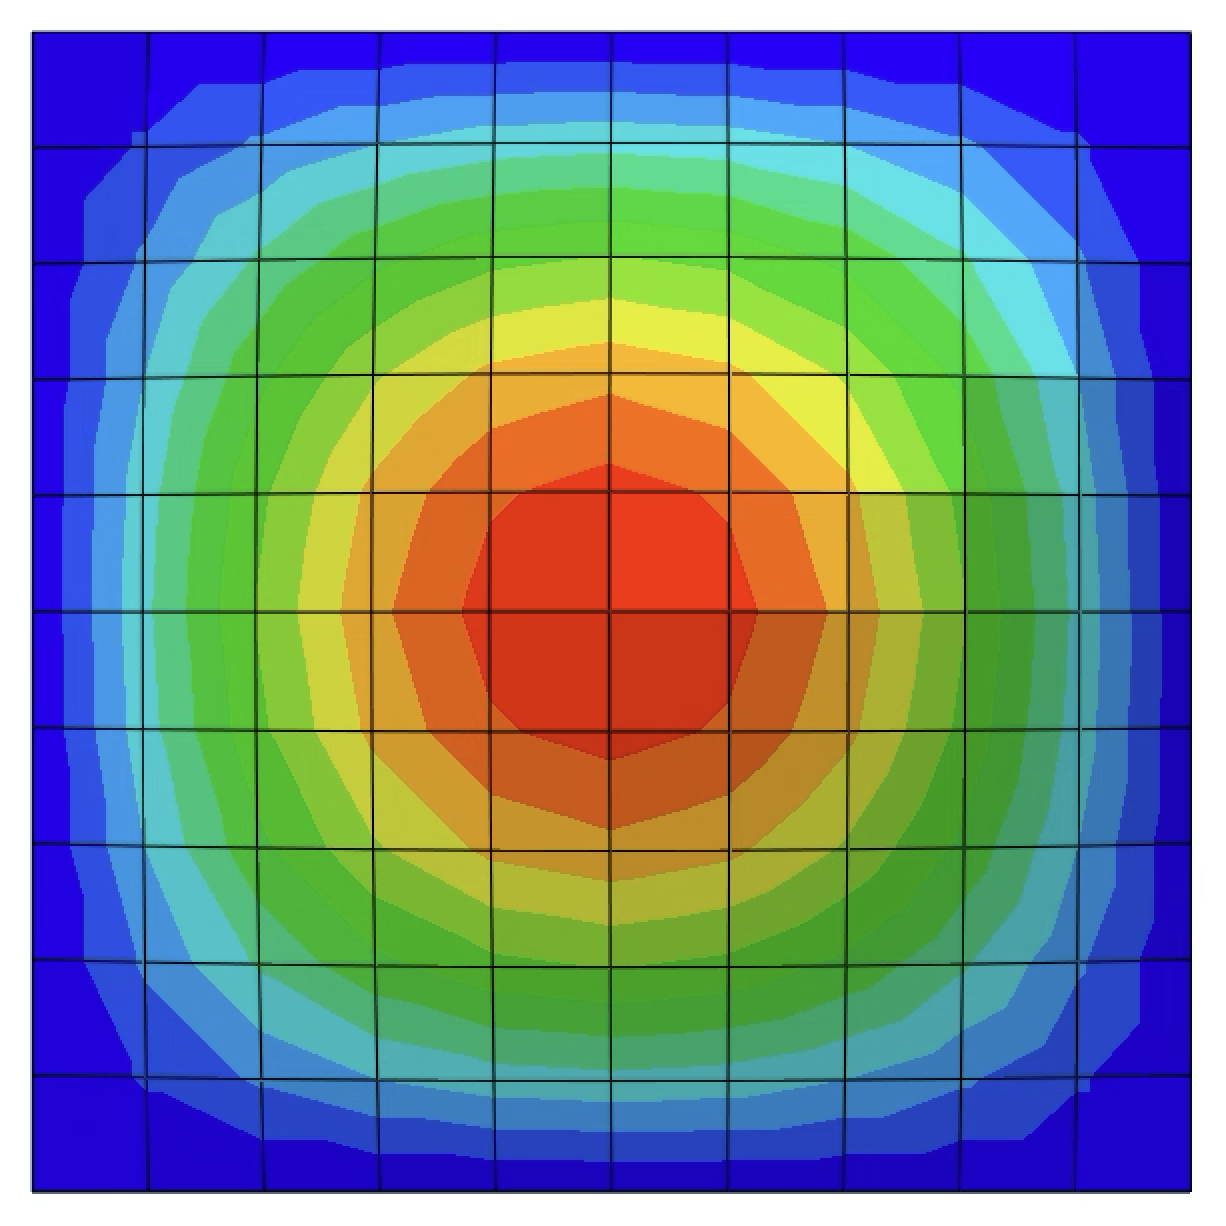
\includegraphics[width=3cm, height=3cm]{../images/thin1.png}
        \caption{Mode shape 1: $\omega_{11}^h=1.001$ Hz}
      \end{subfigure}
      \begin{subfigure}{0.48\textwidth}
        \centering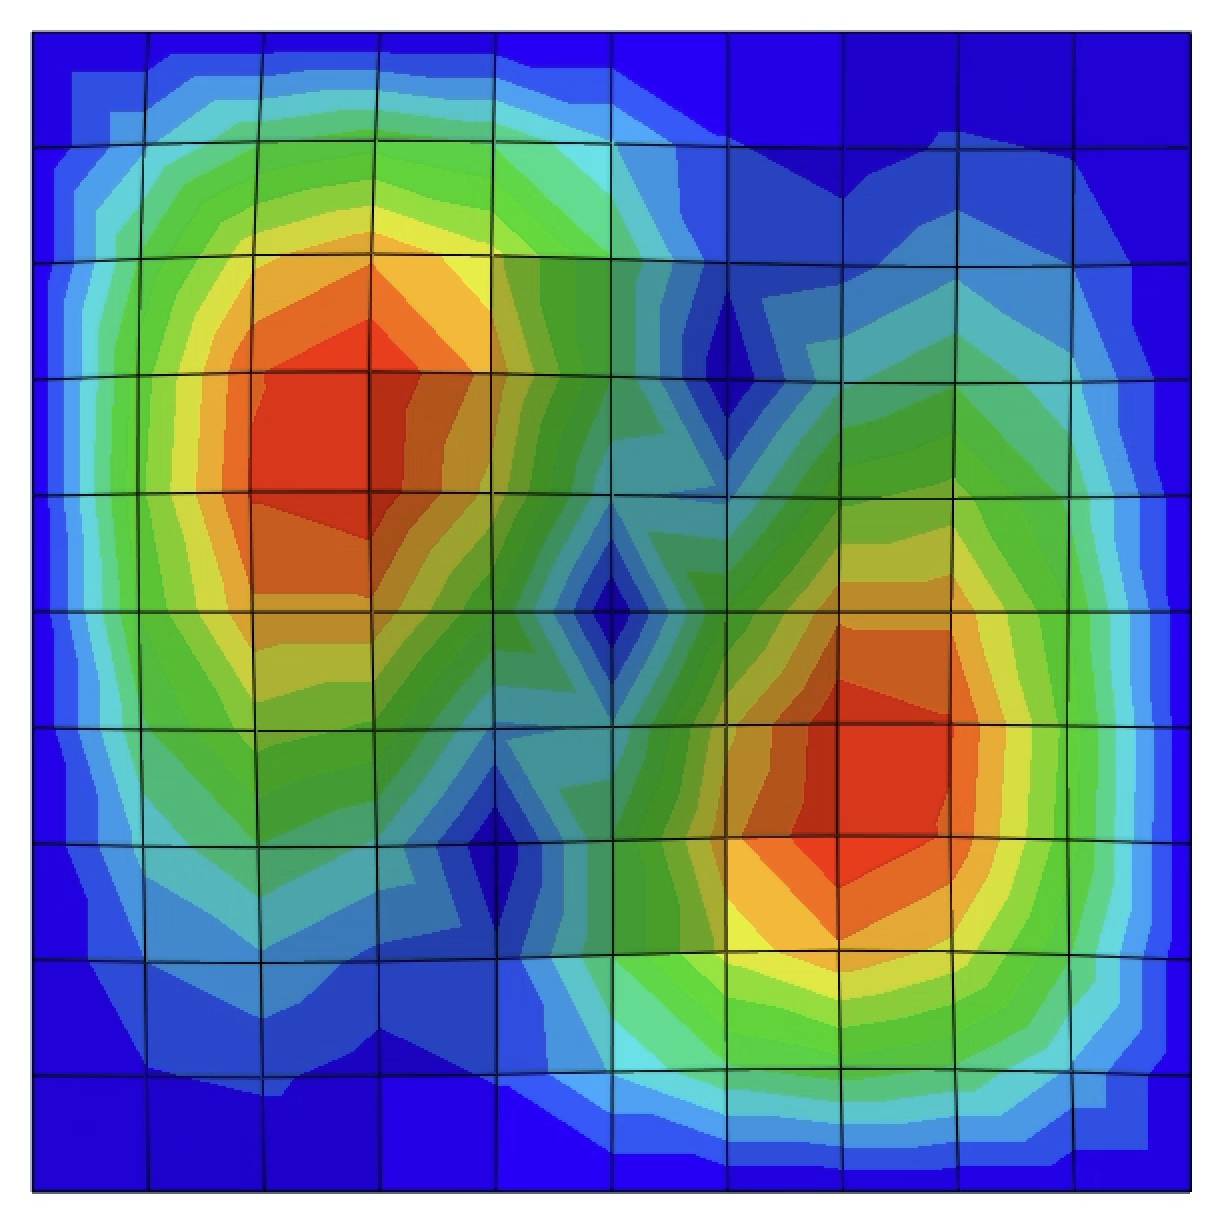
\includegraphics[width=3cm, height=3cm]{../images/thin2.png}
        \caption{Mode shape 2: $\omega_{12}^h=2.573$ Hz}
      \end{subfigure}
      \newline
      \begin{subfigure}{0.48\textwidth}
        \centering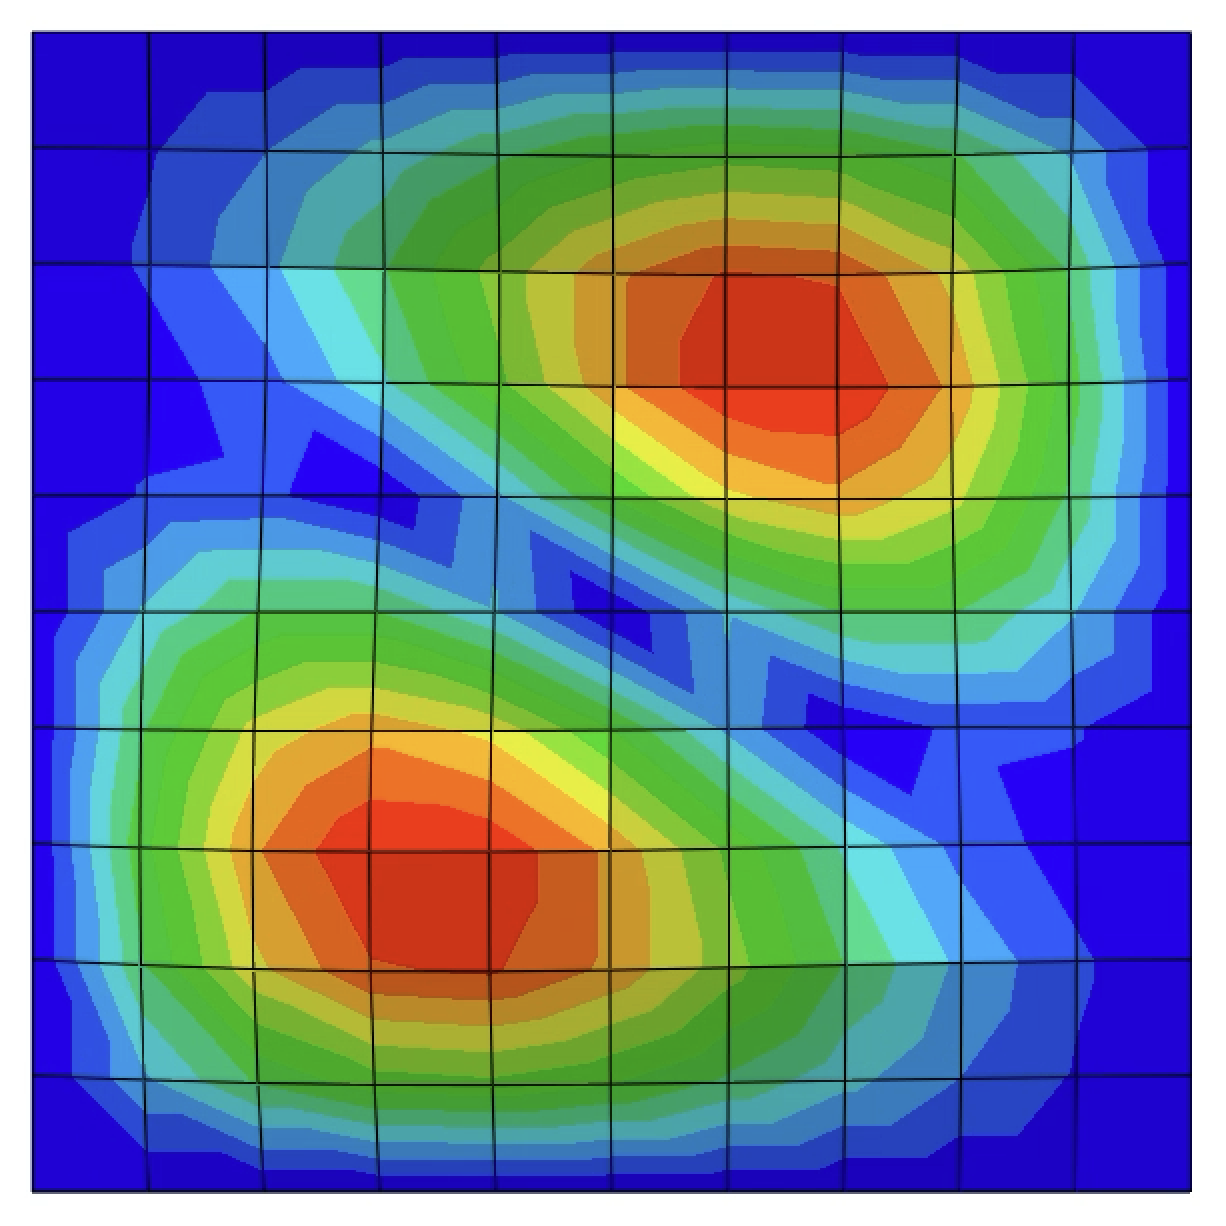
\includegraphics[width=3cm, height=3cm]{../images/thin3.png}
        \caption{Mode shape 3: $\omega_{21}^h=2.573$ Hz}
      \end{subfigure}
      \begin{subfigure}{0.48\textwidth}
        \centering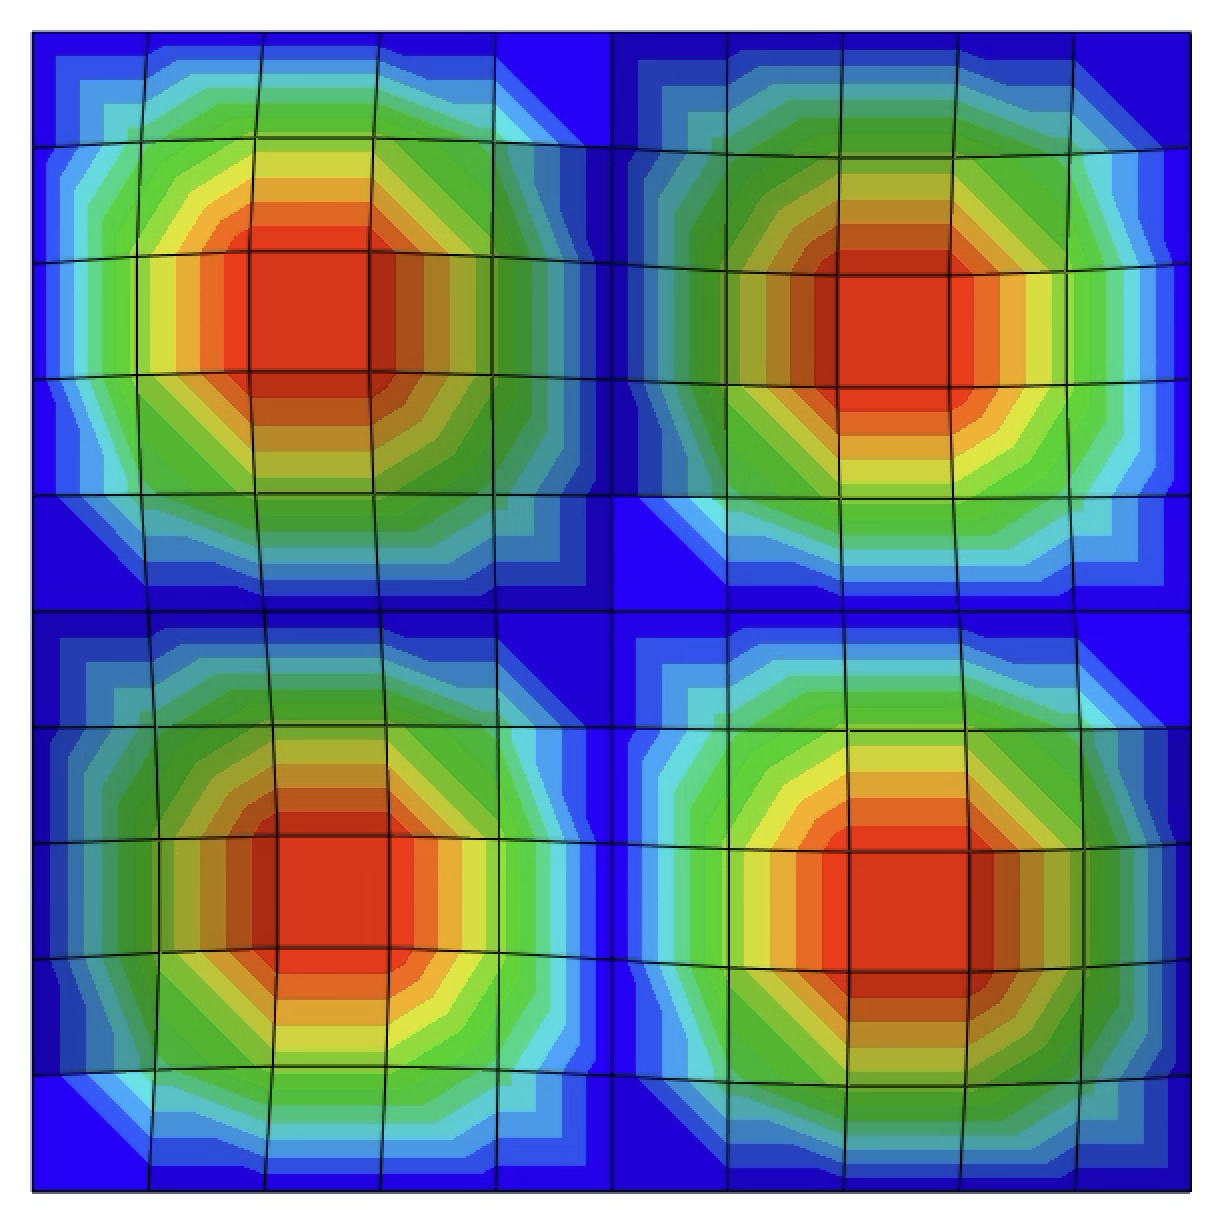
\includegraphics[width=3cm, height=3cm]{../images/thin4.png}
        \caption{Mode shape 4: $\omega_{22}^h=4.103$ Hz}
      \end{subfigure}
    \end{figure}
  \end{frame}
 }

\section{Thin shell elements}

\begin{frame}{Examples of shell structures}
  \begin{columns}
    \begin{column}{0.5\textwidth}
      \begin{center}
        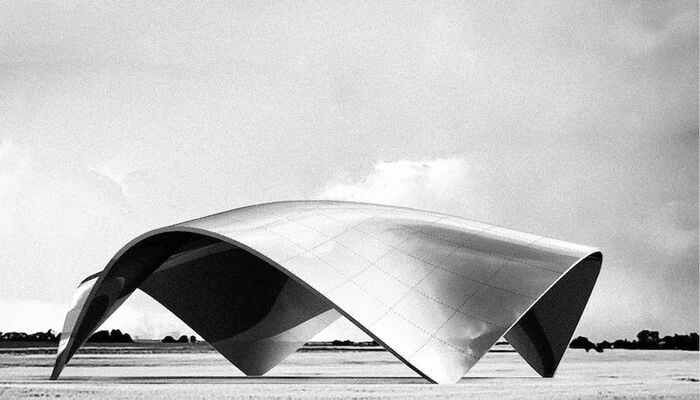
\includegraphics[width=5cm]{../images/shellExample2.jpg}
        \vspace{0.5cm}

        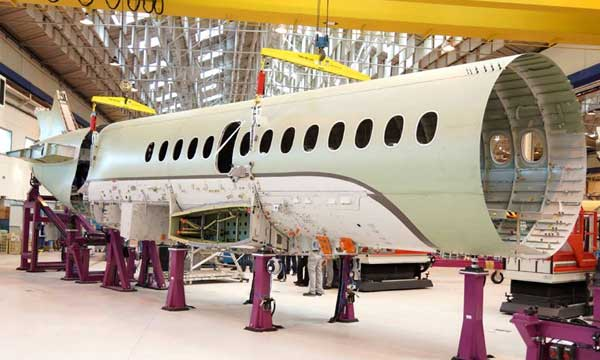
\includegraphics[width=5cm]{../images/shellExample1.jpg}
      \end{center}
    \end{column}
    \begin{column}{0.5\textwidth}
      \begin{center}
        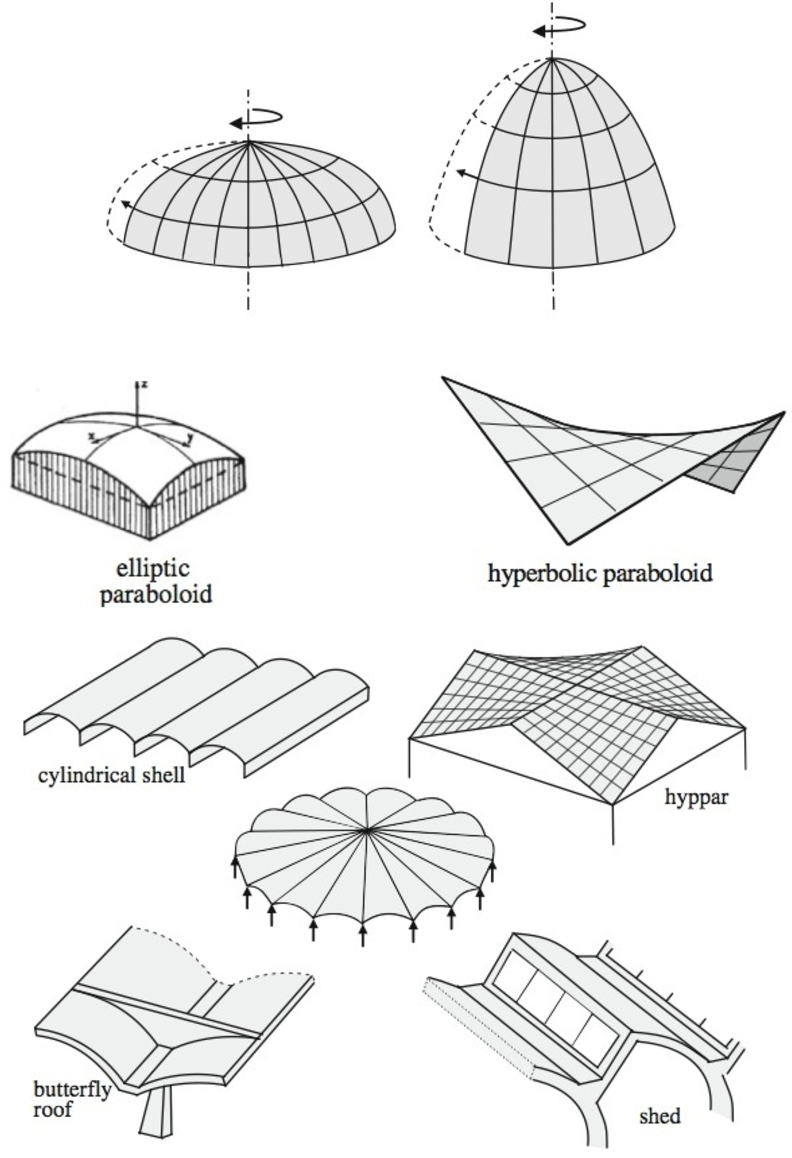
\includegraphics[width=4.5cm]{../images/shellExample3.png}
      \end{center}
    \end{column}
  \end{columns}
\end{frame}

\begin{frame}{Geometry assumptions}
  \begin{tcolorbox}[colback=darkred!10,colframe=darkred!40!black]
    A shell is a three-dimensional curved structural element whose thickness is very small compared to its other two dimensions.
  \end{tcolorbox}
  \begin{itemize}
    \item \textbf{Rectilinearity of transverse fibers} : normals to the middle surface before deformation remain straight during deformation.
    \item \textbf{Inextensibility of transverse fibers}: stress in the normal direction is negligible:
          \vspace{-0.3cm}
          $$\sigma_{33} \approx 0.$$
  \end{itemize}
  \begin{center}
    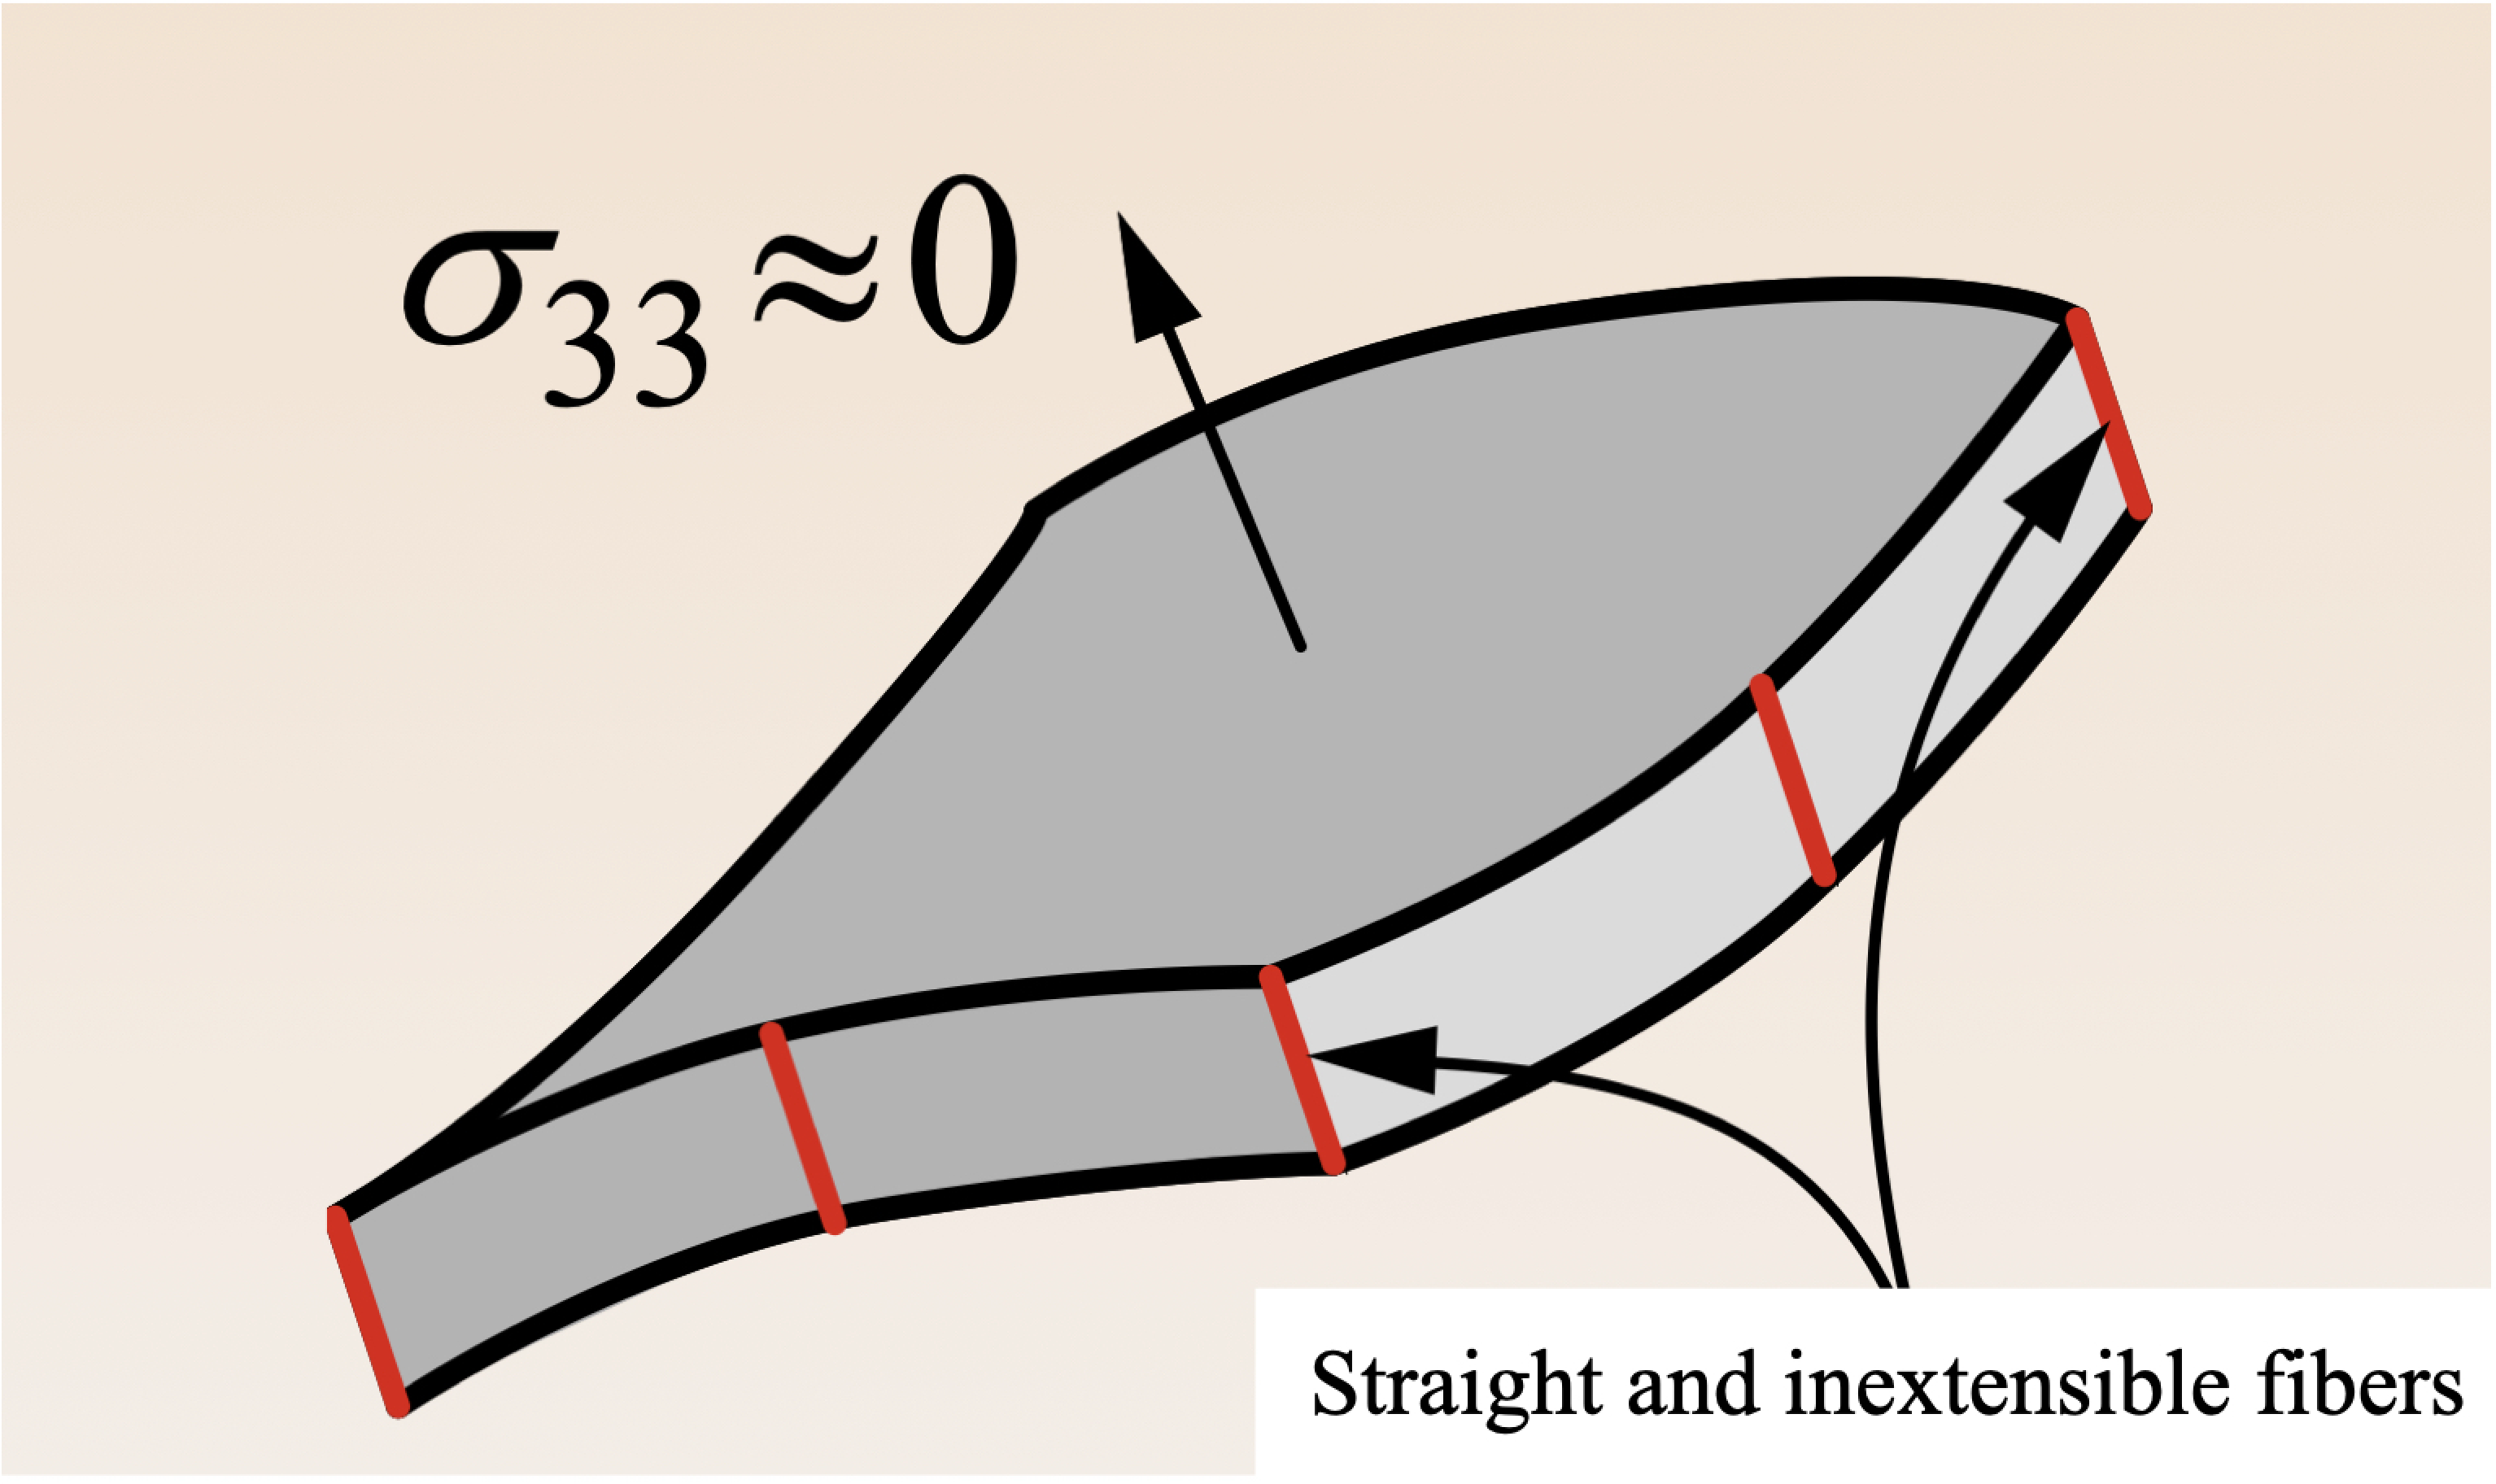
\includegraphics[width=5cm]{../images/shellGeomAssumptions}
  \end{center}
  \emph{\footnotesize (Credit:(G))}
\end{frame}

\begin{frame}{Others $C^0$ shell theories}
  \small
  \begin{itemize}
    \item \textbf{First-Order Shear Deformation Theory (FSDT)}: Accounts for transverse shear deformation by introducing independent rotations, requiring a shear correction factor.
    \item \textbf{Higher-Order Shear Deformation Theory (HSDT)}: Includes higher-order terms in the displacement field to capture transverse shear deformation effects without requiring a shear correction factor.
    \item \textbf{Zig-Zag Theory}: Accounts for the piecewise linear variation of in-plane displacements through the thickness, improving accuracy for layered composites.
  \end{itemize}
  \begin{center}
    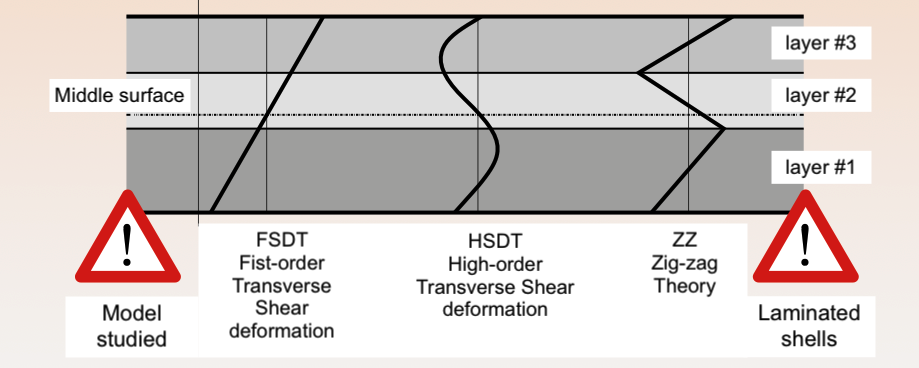
\includegraphics[width=8cm]{../images/shellOtherTheories.png}
  \end{center}
\end{frame}

\begin{frame}{Shell element formulations}
  There are at least three methods of formulating $C^0$ shell elements:
  \begin{enumerate}
    \item Combining a membrane element with a plate bending element to form a \textbf{flat shell element}.
    \item Deriving a curved element using classical \textbf{thin shell theory}.
    \item Deriving a curved element which is a degenerate solid element to form a \textbf{thick shell element}.
  \end{enumerate}
\end{frame}

\begin{frame}{Degenerate solid elements}
  \begin{center}
    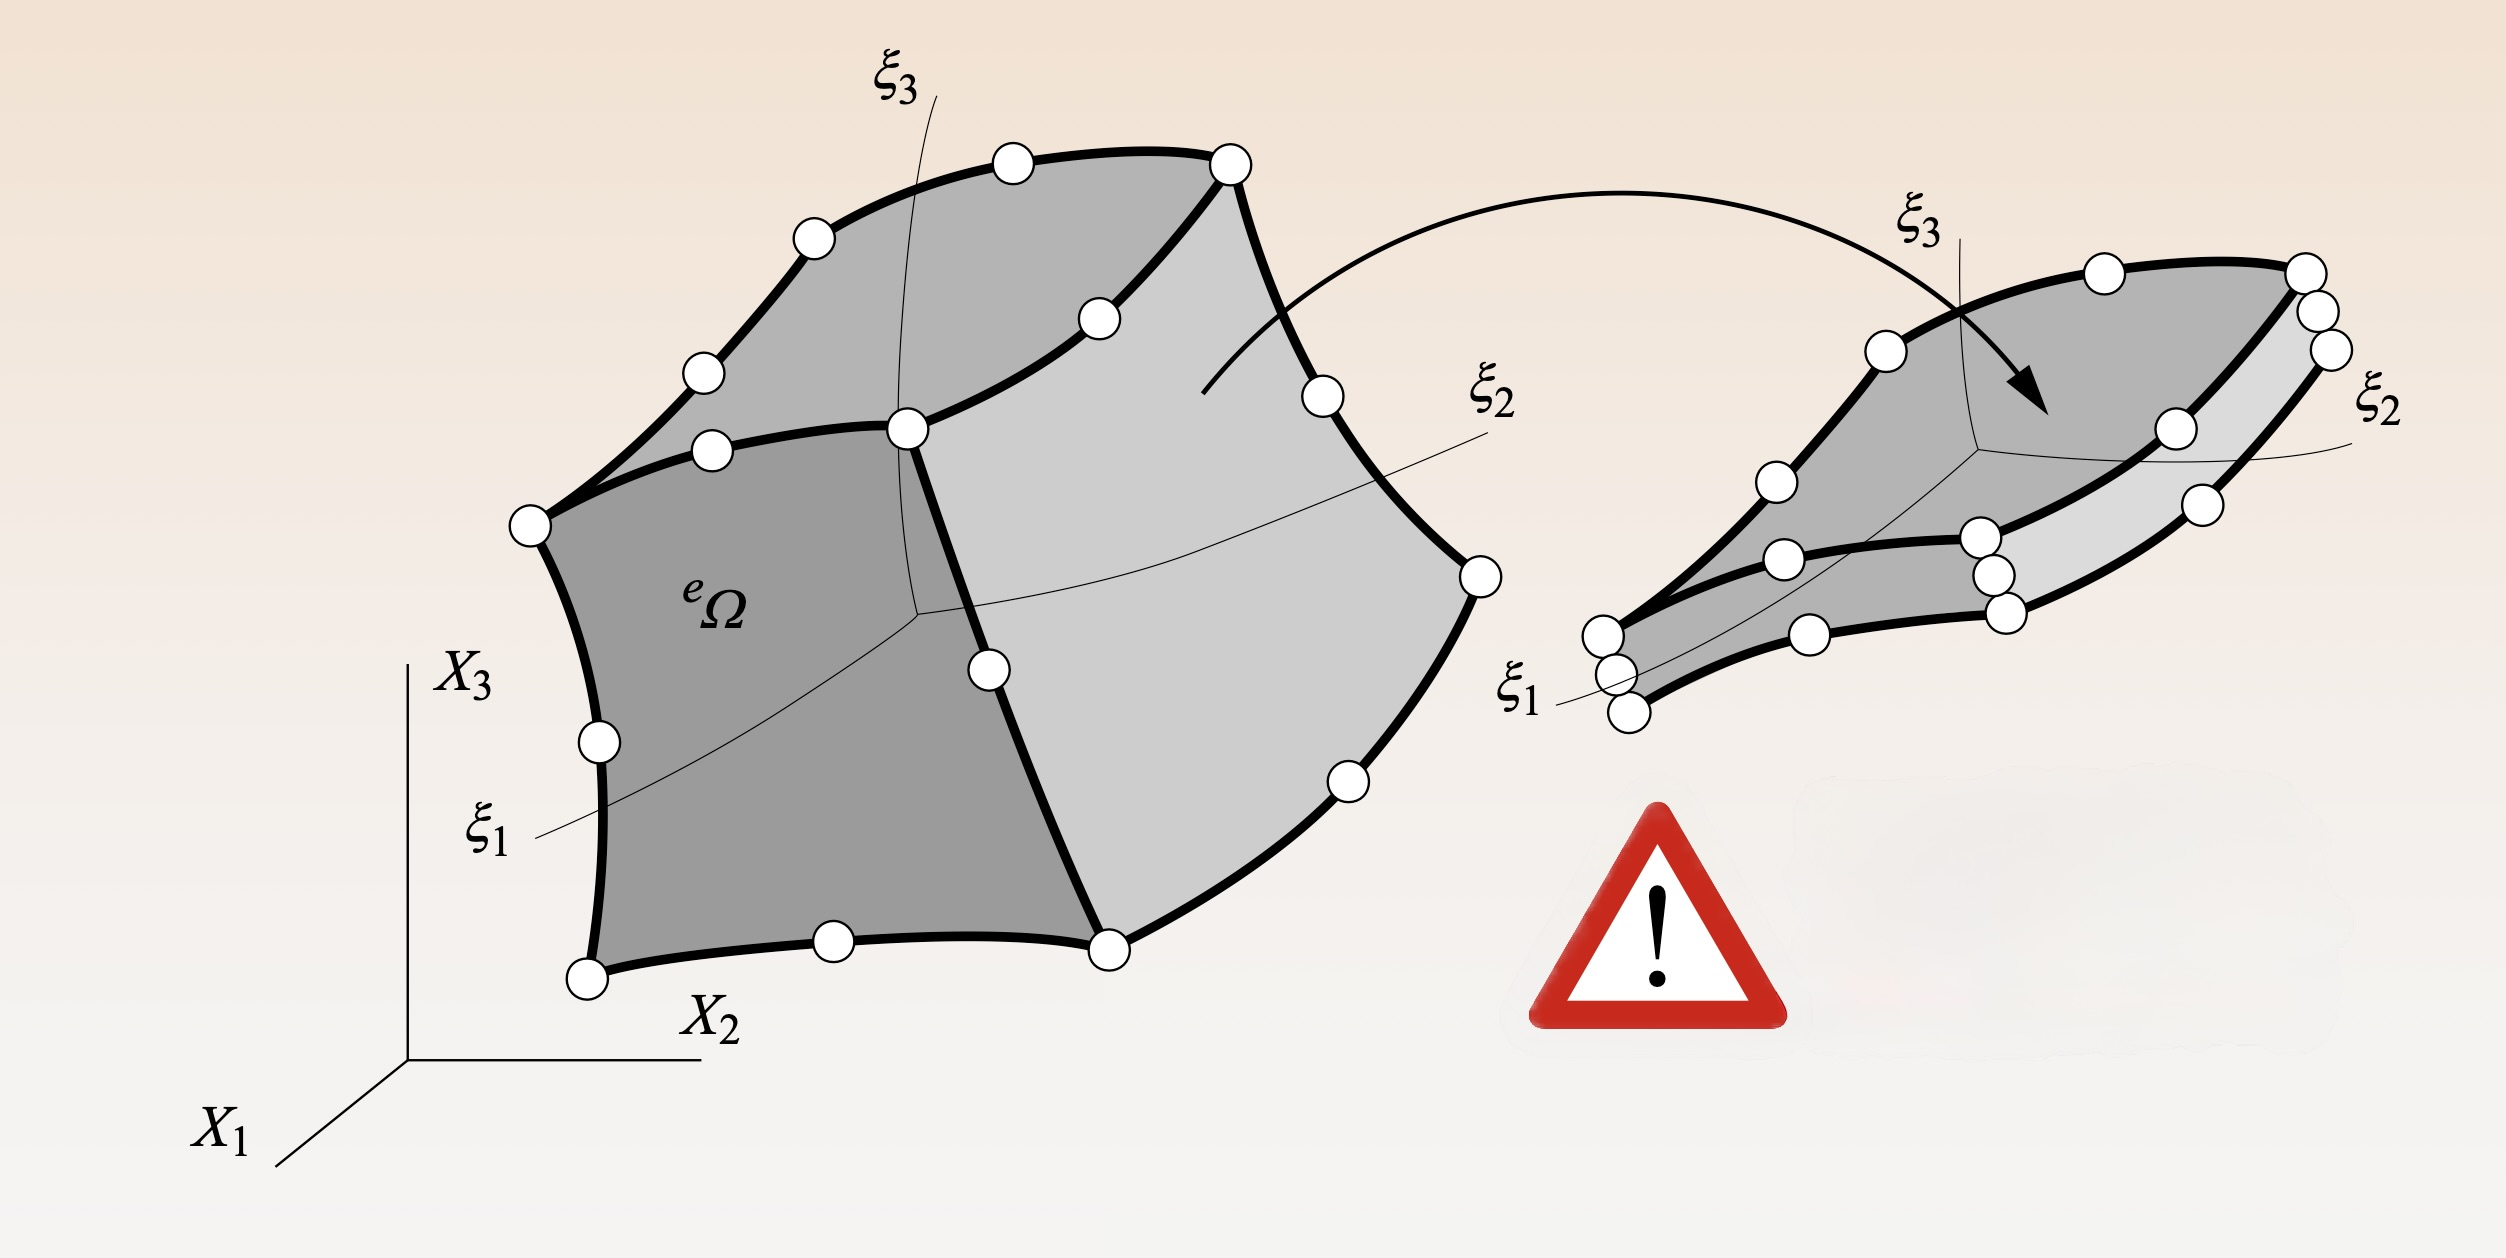
\includegraphics[width=10cm]{../images/shell.jpeg}
  \end{center}
  \begin{itemize}
    \item[\XSolidBrush]  \textbf{Rectilinearity of the transverse fibers hypothesis is not respected}
  \end{itemize}

  \emph{\footnotesize (Credit:(G))}
\end{frame}

\begin{frame}{Thick shell element}
  \begin{center}
    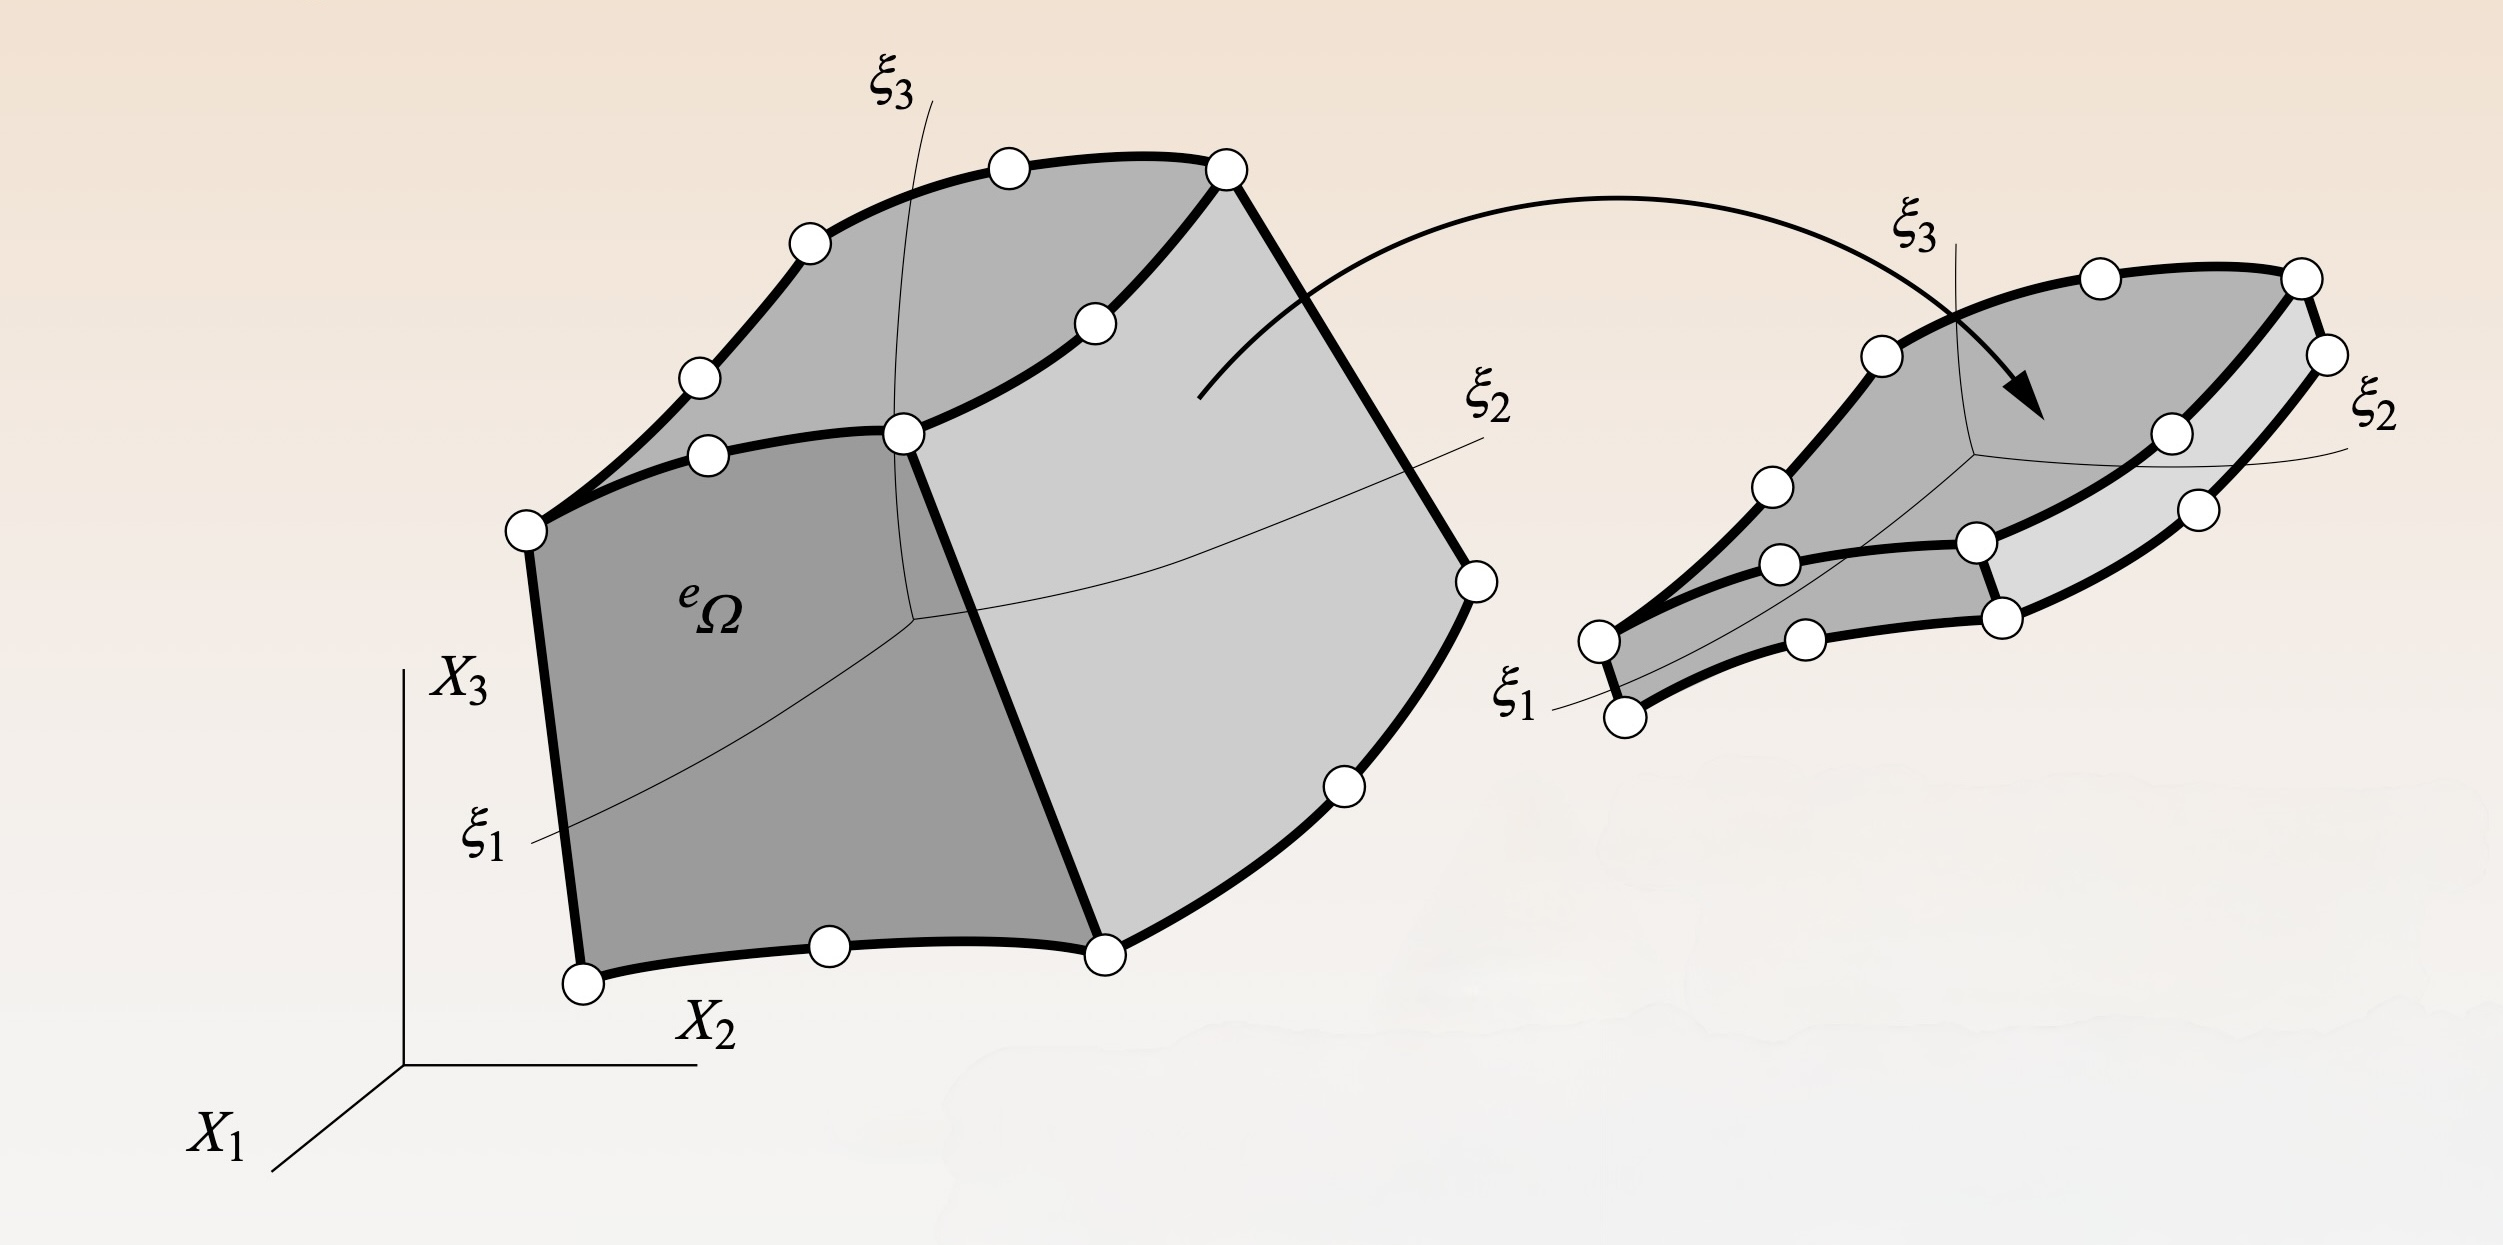
\includegraphics[width=8cm]{../images/shell1.jpeg}
  \end{center}
  \begin{itemize}
    \item Degenerate solid-type shell elements are constructed by modifying three-dimensional solid elements.
    \item Nodes are situated in both the top and the bottom surfaces and have three degrees of freedom each, namely, three components of displacement.
    \item \textbf{Poor conditioning for thin shells due to the excessive deformation.}
  \end{itemize}

  \emph{\footnotesize (Credit:(G))}
\end{frame}

\begin{frame}{Thin shell element}
  \begin{center}
    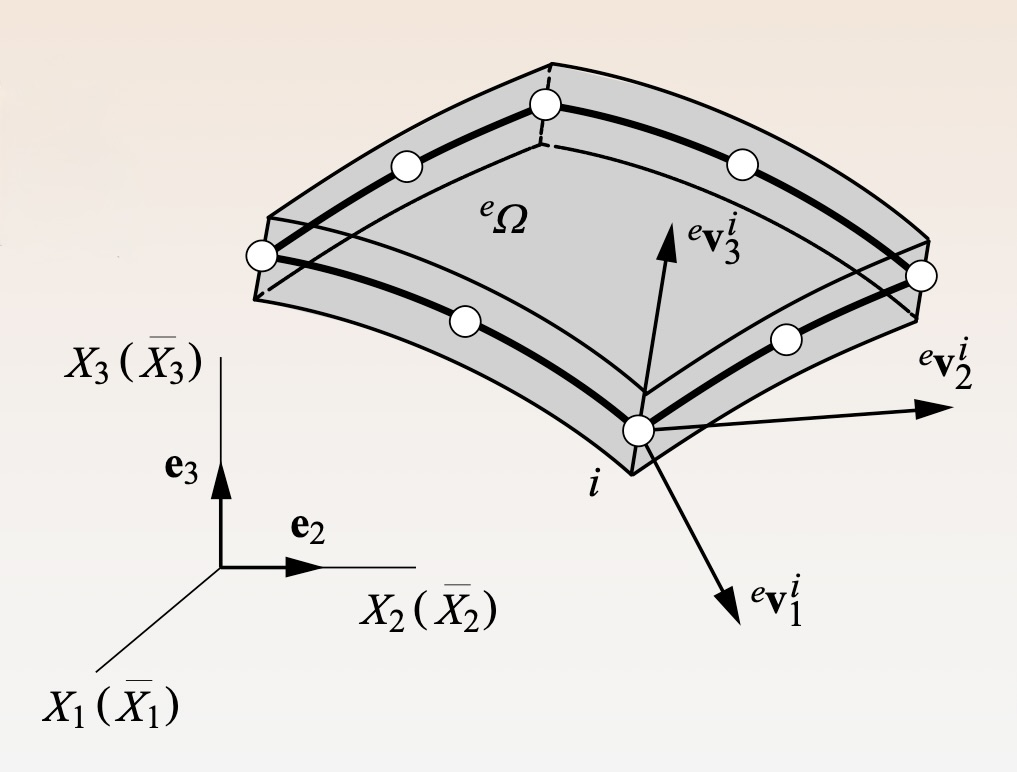
\includegraphics[height=3.5cm]{../images/shellLocalVect.jpeg}
  \end{center}
  \small
  \vspace{-0.3cm}
  \begin{itemize}
    \item   \textbf{Middle surface shell elements} have nodes only in the
          middle surface.
    \item The nodal degrees of freedom consist of three components of displacement and two components of rotation.
    \item These elements are similar to the ones used for thick plate elements.
    \item Superparametric elements : more nodes are required to define the geometry than the deformation.
    \item They can be used to model thin shells provided selective integration is used.
  \end{itemize}
\end{frame}





\begin{frame}{Dyanmic equilibrium equation for thin shells}
  \begin{tcolorbox}[colback=darkred!10,colframe=darkred!40!black]
    The governing equation for thin shell theory is a \emph{reduced} elastodynamic equilibrium equation: $$\nabla^T \overline{\mathbf C}\nabla \mathbf u+\mathbf f=\rho\mathbf{\ddot{u}}\qquad \text{on }\Omega\times]0,T[$$
    where $\Omega$ is characterized by the degenerate hypothesis that one dimension is significantly smaller than the other two.
  \end{tcolorbox}
\end{frame}

\begin{frame}{Elasticity, linearity and isotropic hypothesis}
  \small
  \begin{itemize}
    \item Linear strain-displacement relationship: $\boldsymbol\varepsilon=\nabla\mathbf u$ with
          $$\nabla=\begin{bmatrix} \partial_{x_1} & 0 & 0 \\ 0 & \partial_{x_2} & 0 \\ 0 & 0 & \partial_{x_3} \\ 0 & \partial_{x_3} & \partial_{x_2} \\ \partial_{x_3} & 0 & \partial_{x_1}  \\ \partial_{x_2} & \partial_{x_1} & 0 \end{bmatrix}\qquad\text{and}\qquad \mathbf u=\begin{bmatrix} u_1 \\ u_2 \\ u_3\end{bmatrix}$$
    \item \textbf{Reduced constitutive equation} for isotropic materials: $\boldsymbol\sigma=\overline{\mathbf C}\boldsymbol\varepsilon$:
          $$\overline{\mathbf C}=\frac{E}{1-\nu^2}
            \begin{bmatrix}
              1   & \nu & 0 & 0         & 0          & 0          \\
              \nu & 1   & 0 & 0         & 0          & 0          \\
              0   & 0   & 0 & 0         & 0          & 0          \\
              0   & 0   & 0 & (1-\nu)/2 & 0          & 0          \\
              0   & 0   & 0 & 0         & k(1-\nu)/2 & 0          \\
              0   & 0   & 0 & 0         & 0          & k(1-\nu)/2 \\
            \end{bmatrix}$$
          $E$ is the Young's modulus, $\nu$ is the Poisson's ratio, and $k$ is the shear correction factor.
  \end{itemize}
\end{frame}


\begin{frame}{Coordinate transformation}
  Finite solid element with linear edges along the $\xi_3$ direction.
  \begin{center}
    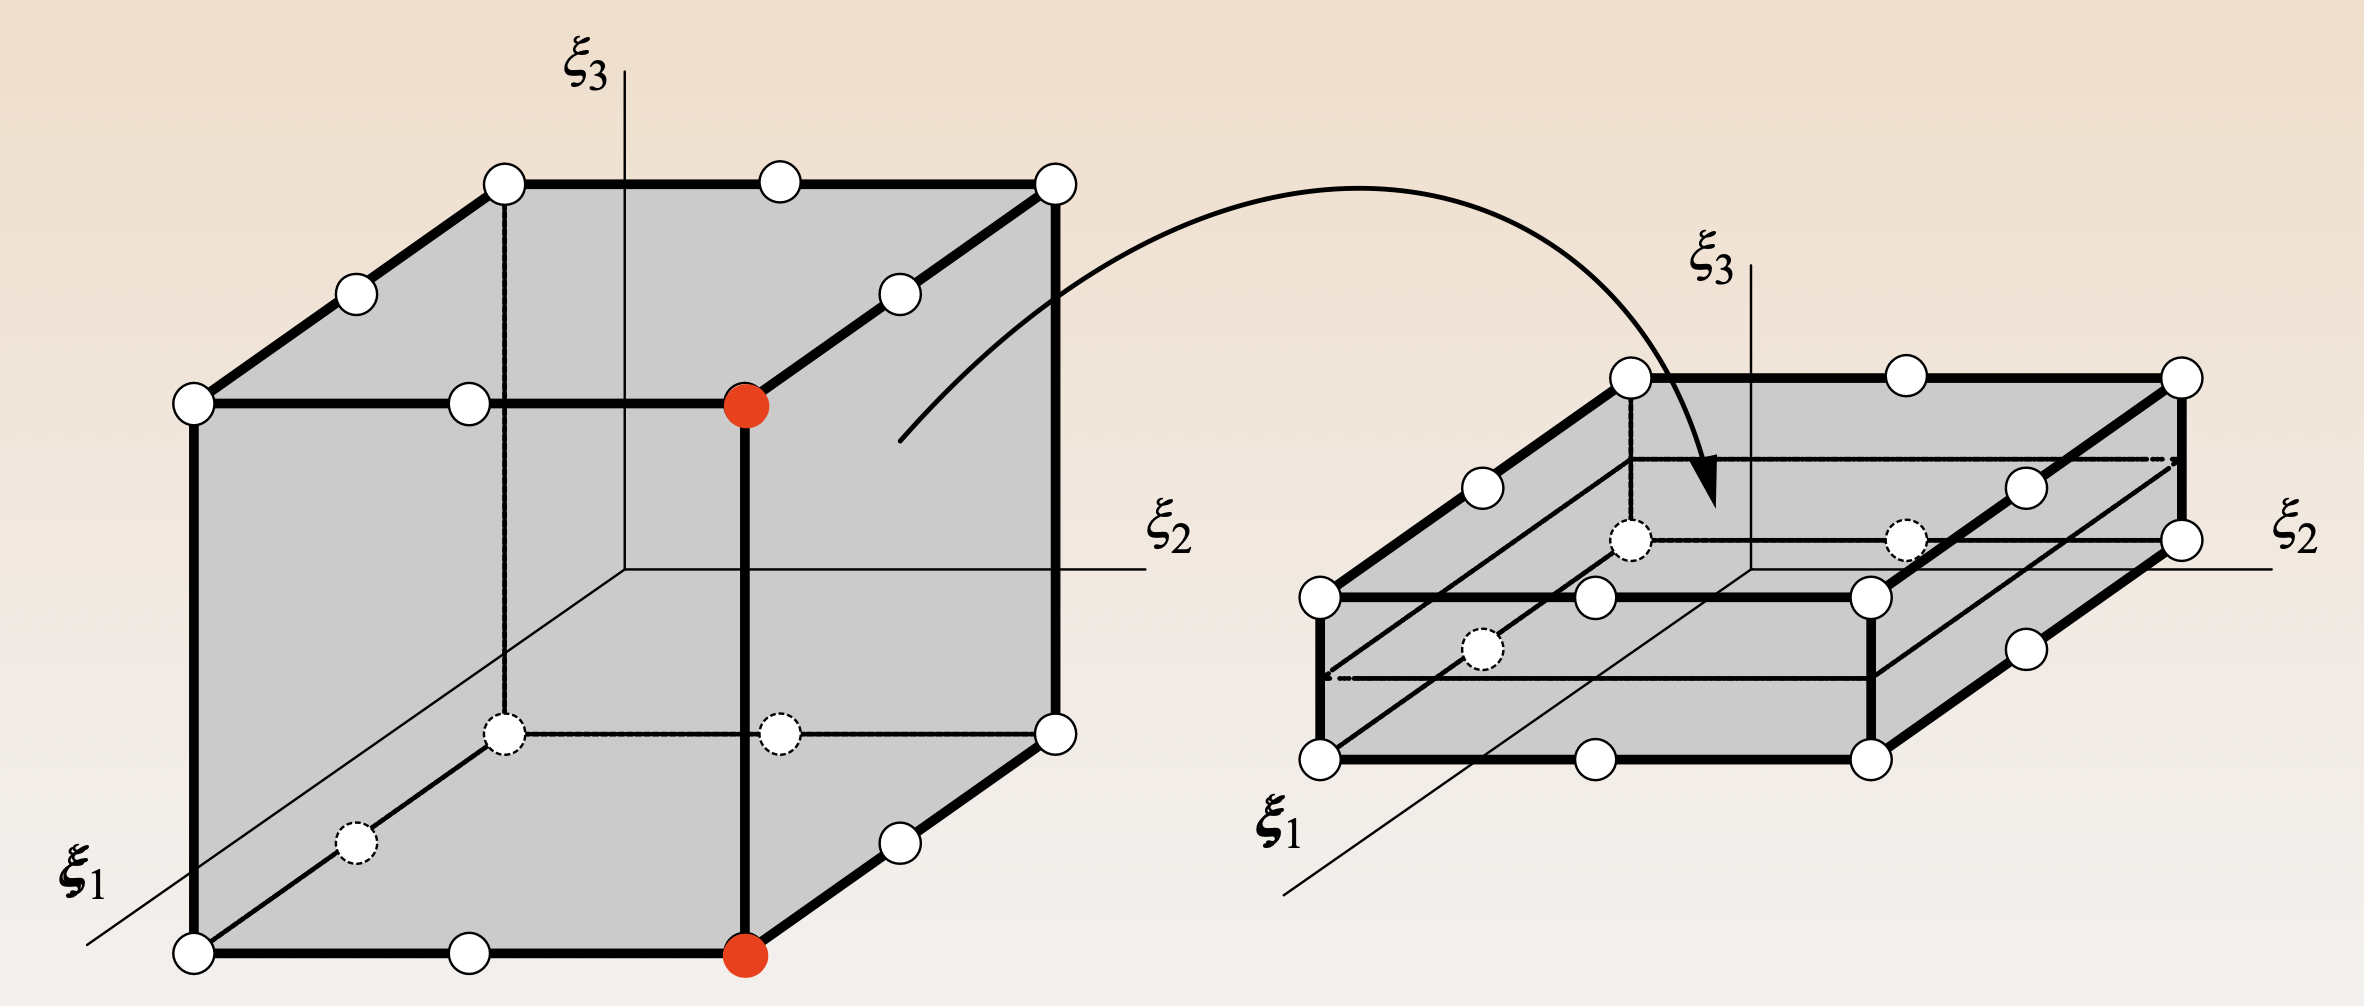
\includegraphics[height=3cm]{../images/shell2.png}
    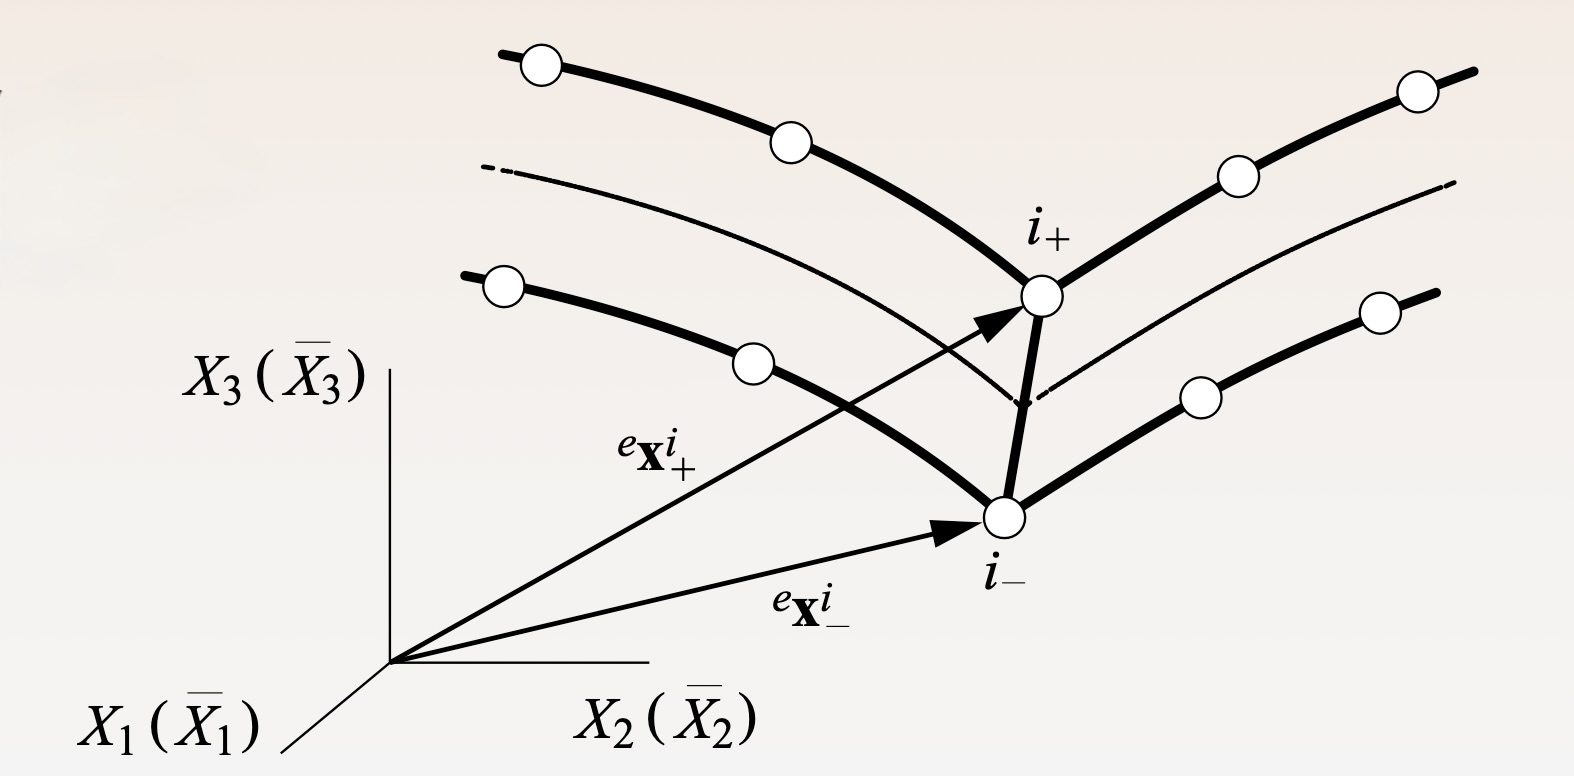
\includegraphics[height=3cm]{../images/shell3.jpeg}
  \end{center}
  Nodes on top and bottom faces in pairs. Let ${}^eq$ be the total number of nodes.
  \begin{block}{}
    $${}^eT:\quad \mathbf x(\boldxi)=\sum_{i=1}^{{}^eq/2}{}^ah_i(\xi_1,\xi_2)\left[\frac{1-\xi_3}{2}{}^e\mathbf x_-^i+\frac{1+\xi_3}{2}{}^e\mathbf x_+^i\right]$$
  \end{block}
  ${}^e\mathbf x_-^i$ and ${}^e\mathbf x_+^i$ are the coordinates of node $i$ on the bottom and top faces respectively.
\end{frame}

\begin{frame}{Coordinate transformation}
  \vspace{-0.3cm}
  \begin{columns}
    \begin{column}{.6\textwidth}
      \begin{center}
        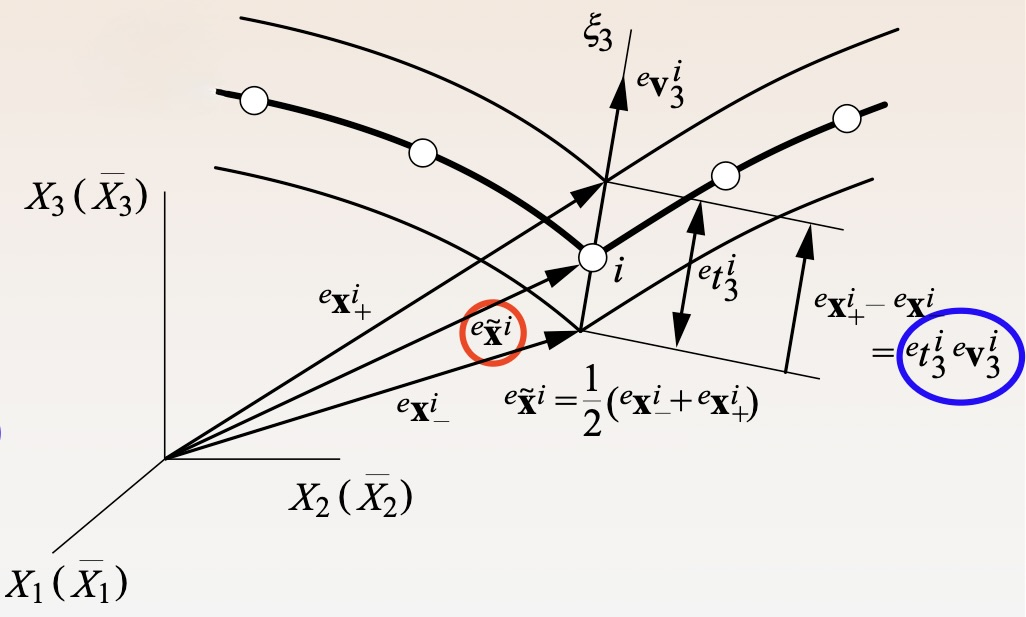
\includegraphics[height=4.4cm]{../images/shell4.jpeg}
      \end{center}
    \end{column}
    \begin{column}{.4\textwidth}
      \vspace{0.2cm}

      Let ${}^ep={}^eq/2$ be the total number of nodes on the midsurface.
      \begin{itemize}
        \item[${}^e\tilde{\mathbf x}^i$] coordinate of node $i$ on the midsurface of ${}^e\Omega$
        \item[${}^et^i_3$] thickness at node $i$
        \item[${}^e{\mathbf v}_3^i$] normal vector to the midsurface at node $i$
      \end{itemize}
    \end{column}
  \end{columns}
  \begin{block}{}\vspace{-0.5cm}
    \begin{align*}
      {}^eT: \mathbf x(\boldxi) & =\sum_{i=1}^{{}^ep}{}^ah_i(\xi_1,\xi_2)\left[\frac{1}{2}({}^e\mathbf x_-^i+{}^e\mathbf x_+^i)+\frac{1}{2}\xi_3 ({}^e\mathbf x_-^i-{}^e\mathbf x_+^i)\right] \\
                                & =\sum_{i=1}^{{}^ep}{}^ah_i(\xi_1,\xi_2)\left[{}^e\tilde{\mathbf x}^i+\frac{1}{2}\xi_3{}^e t_3^i {}^e\mathbf v_3^i\right]
    \end{align*}
  \end{block}
\end{frame}

\begin{frame}{Approximate displacements}
  Analogy with transformation of coordinates:
  \begin{block}{}%\vspace{-0.5cm}
    $$\mathbf u^h(\boldxi)  =\sum_{i=1}^{{}^ep}{}^ah_i(\xi_1,\xi_2)\left[{}^e{\mathbf d}^i+\frac{1}{2}\xi_3{}^e t_3^i\left(-{}^e\theta_1^i{}^e\mathbf v_2^i+{}^e\theta_2^i{}^e\mathbf v_1^i\right)\right]
    $$
  \end{block}
  \vspace{-0.2cm}
  \begin{columns}
    \begin{column}{.6\textwidth}
      \begin{center}
        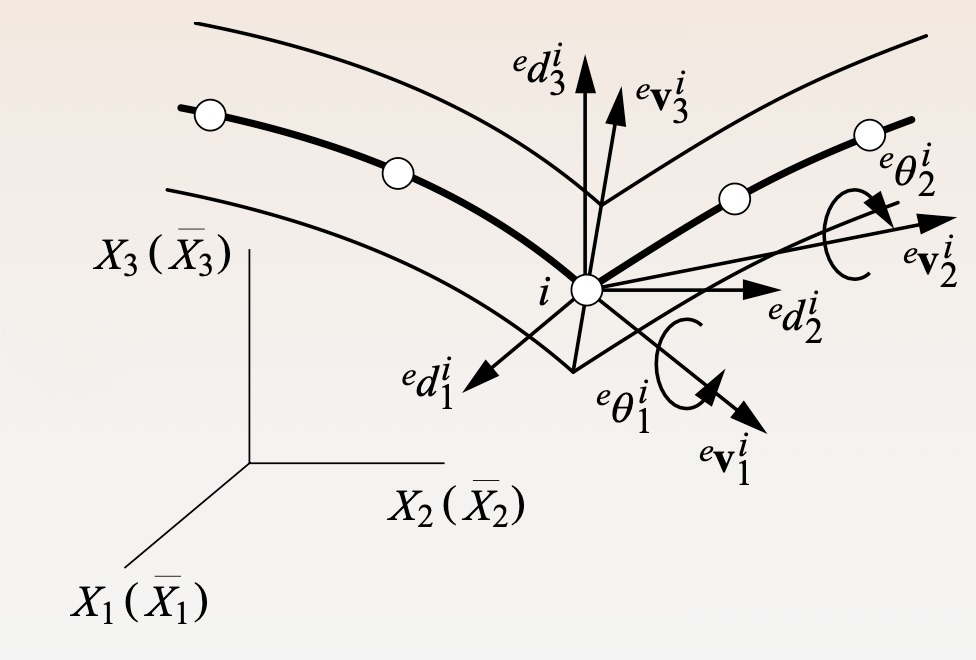
\includegraphics[height=5cm]{../images/shell5.jpeg}
      \end{center}
    \end{column}
    \begin{column}{.45\textwidth}
      $${}^e{\mathbf d}^i=[{}^e{d}^i_1,{}^e{d}^i_2,{}^e{d}^i_3]^T$$
      \vspace{-0.5cm}
      \begin{itemize}
        \item ${}^e{d}^i_1,{}^e{d}^i_2,{}^e{d}^i_3$ displacements of node $i$, oriented along the \emph{global axis}.
        \item ${}^e{\theta}^i_1,{}^e{\theta}^i_2$ rotations of node $i$, oriented along the \emph{local axis}:
              \begin{itemize}
                \item ${}^e{\theta}^i_1$ rotation about ${}^e\mathbf v_1^i$.
                \item ${}^e{\theta}^i_2$ rotation about ${}^e\mathbf v_2^i$.
              \end{itemize}
      \end{itemize}
    \end{column}
  \end{columns}
\end{frame}


\begin{frame}{Construction of local vectors}
  \vspace{-0.2cm}
  \begin{columns}
    \begin{column}{.5\textwidth}
      \begin{itemize}
        \item We have:
              $${}^e\mathbf v^i_3={}^e\mathbf x_-^i-{}^e\mathbf x_+^i$$ the normal vector to the midsurface at node $i$.
        \item We define the local vectors:
              \begin{align*}
                {}^e\mathbf v^i_1 & =\begin{cases}
                                       \mathbf e_2\wedge {}^e\mathbf v^i_3 & \text{if } {}^e\mathbf v^i_3\neq \pm \mathbf e_2 \\
                                       \pm \mathbf e_3                     & \text{if } {}^e\mathbf v^i_3= \pm \mathbf e_2\end{cases} \\
                {}^e\mathbf v^i_2 & ={}^e\mathbf v^i_3\wedge {}^e\mathbf v^i_1
              \end{align*}
      \end{itemize}
    \end{column}
    \begin{column}{.45\textwidth}
      \begin{center}
        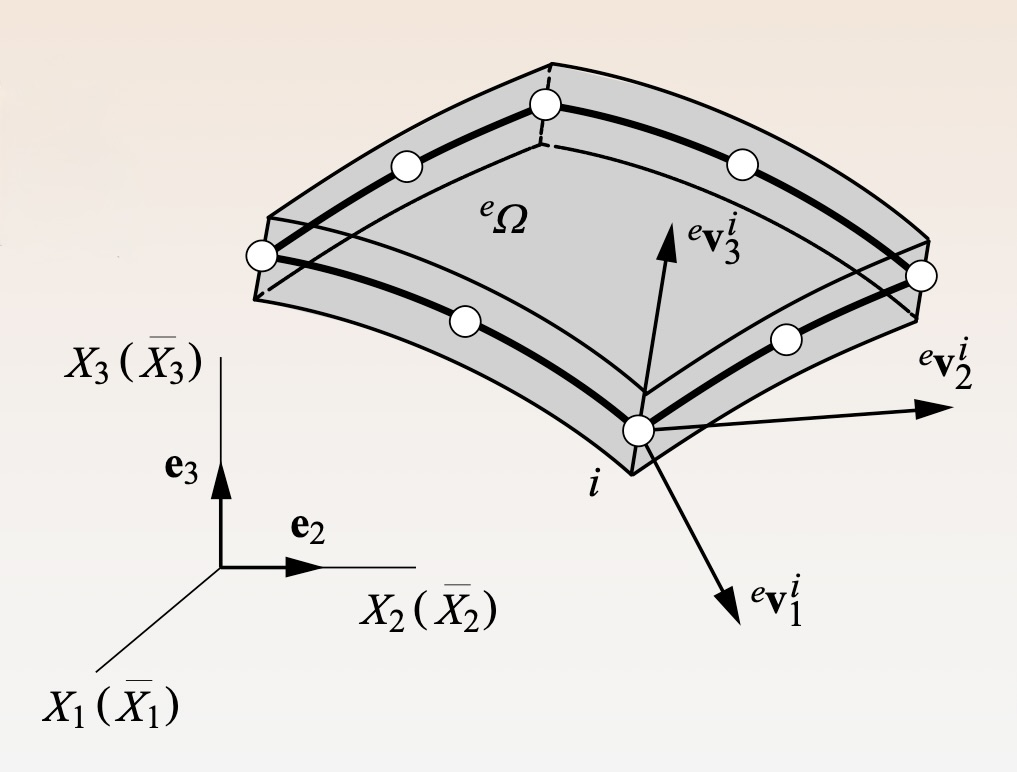
\includegraphics[height=5cm]{../images/shellLocalVect.jpeg}
      \end{center}
    \end{column}
  \end{columns}
\end{frame}

\begin{frame}{Thin shell elements}
  \begin{center}
    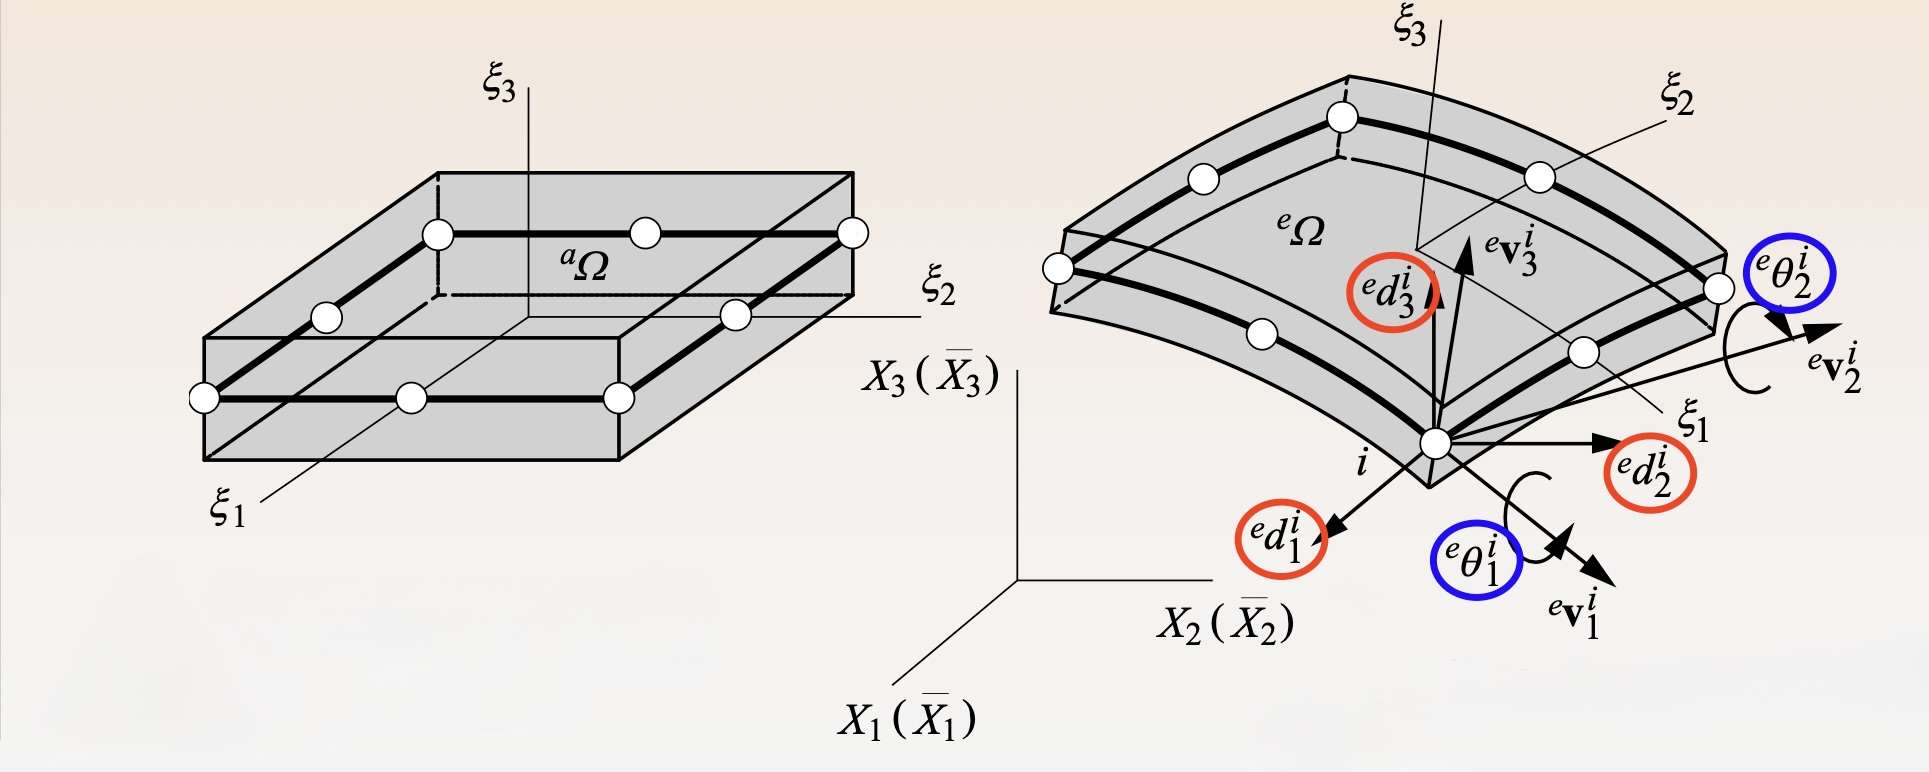
\includegraphics[height=4cm]{../images/shell6.jpeg}
  \end{center}
  \begin{itemize}
    \item[\Checkmark] 5 DOFs per node, no rotation ${}^e\theta_3^i$ w.r.t the normal local vector ${}^e\mathbf v_3^i$.
    \item[\Checkmark] Lead to huge computational time savings since allow modeling with fewer nodes.
    \item[\Checkmark] Less prone to negative Jacobian errors which might occur when using extremely thin 3d solid elements.
  \end{itemize}
\end{frame}


{\setbeamercolor{background canvas}{bg=darkred}
\setbeamercolor{block body}{bg=darkred,fg=white}
\setbeamercolor{itemize item}{fg=white}
\setbeamercolor{itemize/enumerate body}{fg=white}
\color{white}
\begin{frame}{Shape functions matrix}
  \begin{block}{}\vspace{-0.5cm}
    \begin{align*}
      \mathbf u^h(\boldxi) & =\sum_{i=1}^{{}^ep}{}^ah_i(\xi_1,\xi_2)\left[{}^e{\mathbf d}^i+\frac{1}{2}\xi_3{}^e t_3^i\left(-{}^e\theta_1^i{}^e\mathbf v_2^i+{}^e\theta_2^i{}^e\mathbf v_1^i\right)\right] \\[10pt]
                           & =\sum_{i=1}^{{}^ep}{}^a\mathbf H_i(\boldxi){}^e\mathbf q^i(t)                                                                                                                 \\[10pt]
                           & =\sum_{i=1}^{{}^ep}\underbrace{\left[
          \begin{array}{ccc|cc}
            {}^a h_i                                                 & 0                                                       & 0        &
            -\dfrac{1}{2}\xi_3{}^e t_3^i \, {}^a h_i \, {}^ev_{21}^i & \dfrac{1}{2}\xi_3{}^e t_3^i \, {}^a h_i \, {}^ev_{11}^i                                                                                                                             \\[7pt]
            0                                                        & {}^a h_i                                                & 0        & -\dfrac{1}{2}\xi_3{}^e t_3^i \, {}^a h_i \, v_{22}^i & \dfrac{1}{2}\xi_3{}^e t_3^i \, {}^a h_i \, {}^ev_{12}^i \\[7pt]
            0                                                        & 0                                                       & {}^a h_i &
            -\dfrac{1}{2}\xi_3{}^e t_3^i \, {}^a h_i \, {}^ev_{23}^i & \dfrac{1}{2}\xi_3{}^e t_3^i \, {}^a h_i  \,{}^ev_{13}^i
          \end{array}
          \right]}_\text{${}^a\mathbf H_i$}
      \underbrace{\begin{bmatrix}
                      {}^e{d}^i_1 \\[2pt] {}^e{d}^i_2 \\[2pt] {}^e{d}^i_3 \\[2pt] {}^e{\theta}^i_1 \\[2pt] {}^e{\theta}^i_2
                    \end{bmatrix}}_\text{${}^e\mathbf q^i$}
    \end{align*}
  \end{block}
\end{frame}

\begin{frame}{Deformation matrix}
  \begin{block}{}\vspace{-0.5cm}
    \begin{align*}
      {}^a\mathbf B_i = & \nabla {}^a\mathbf H_i \\
      =                 & \left[
        \begin{array}{ccccc}
          \frac{\partial {}^eh_i}{\partial x_1} & 0                                     & 0                                     & {}^eg_{11}^i                & {}^ef_{11}^i                \\[10pt]
          0                                     & \frac{\partial{}^e h_i}{\partial x_2} & 0                                     & {}^eg_{22}^i                & {}^ef_{22}^i                \\[10pt]
          0                                     & 0                                     & \frac{\partial {}^eh_i}{\partial x_3} & {}^eg_{33}^i                & {}^ef_{33}^i                \\[10pt]
          0                                     & \frac{\partial {}^eh_i}{\partial x_3} & \frac{\partial {}^eh_i}{\partial x_2} & {}^eg_{23}^i + {}^eg_{32}^i & {}^ef_{23}^i + {}^ef_{32}^i \\[10pt]
          \frac{\partial {}^eh_i}{\partial x_3} & 0                                     & \frac{\partial {}^eh_i}{\partial x_1} & {}^eg_{31}^i + {}^eg_{13}^i & {}^ef_{31}^i + {}^ef_{13}^i \\[10pt]
          \frac{\partial{}^e h_i}{\partial x_2} & \frac{\partial{}^e h_i}{\partial x_1} & 0                                     & {}^eg_{12}^i + {}^eg_{21}^i & {}^ef_{12}^i + {}^ef_{21}^i
        \end{array}
        \right]
      \qquad (i = 1, 2, \dots, {}^ep)
    \end{align*}
  \end{block}
\end{frame}
}

\begin{frame}{Deformation matrix}
  Derivative with respect to global variables:
  \[
    \frac{\partial {}^eh_i}{\partial x_k}
    = \frac{\partial {}^ah_i}{\partial \xi_1} \frac{\partial \xi_1}{\partial x_k}  + \frac{\partial {}^ah_i}{\partial \xi_2}\frac{\partial \xi_2}{\partial x_k}={}^eJ^{-1}_{k1} \frac{\partial {}^ah_i}{\partial \xi_1}
    + {}^eJ^{-1}_{k2} \frac{\partial {}^ah_i}{\partial \xi_2}
  \]
  and
  \begin{align*}
    {}^ef_{jk}^{i}  & = \frac{1}{2} \, {}^et_3^i v_{1j}^{i}\frac{\partial (\xi_3 \, {}^e h_i)}{\partial x_k},     \\
    {}^e g_{jk}^{i} & = -\frac{1}{2}  \, {}^et_3^i v_{2j}^{i}\, \frac{\partial (\xi_3 \, {}^e h_i)}{\partial x_k} \\
    \frac{\partial(\xi_3 \, {}^eh_i)}{\partial x_k}
                    & = \xi_3  \frac{\partial {}^eh_i}{\partial x_k}
    + {}^ah_i \frac{\partial \xi_3}{\partial x_k}=\xi_3  \left(
    {}^eJ^{-1}_{k1} \frac{\partial {}^ah_i}{\partial \xi_1}
    + {}^eJ^{-1}_{k2} \frac{\partial {}^ah_i}{\partial \xi_2}
    \right)
    + {}^eJ^{-1}_{k3} {}^ah_i
  \end{align*}
\end{frame}

\begin{frame}{Examples of thin shell elements}
  Along the midsurface of the shell we can use Lagrangian 2D finite elements such as, for example, bicubic quadrilateral or bicubic triangular elements.
  \begin{columns}
    \begin{column}{.48\textwidth}
      \begin{center}
        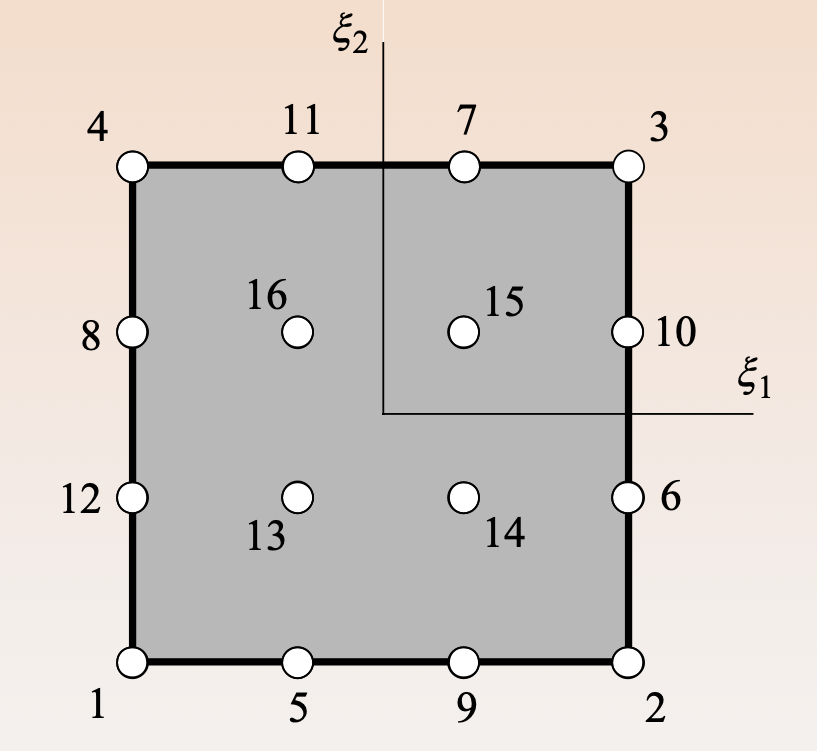
\includegraphics[height=5cm]{../images/shellQuad.png}
      \end{center}
    \end{column}
    \begin{column}{.48\textwidth}
      \begin{center}
        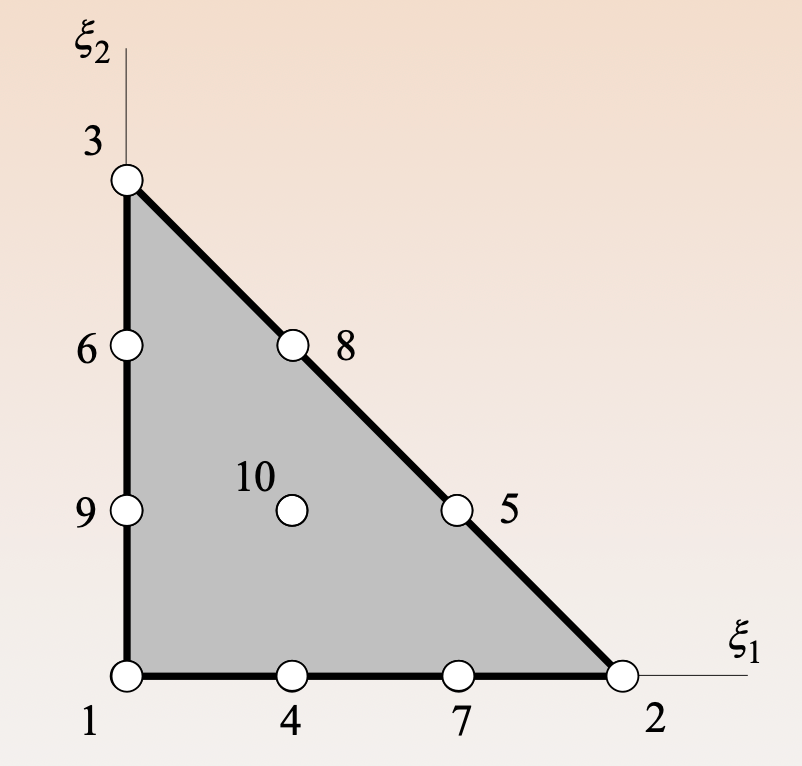
\includegraphics[height=5cm]{../images/ShellTrg.png}
      \end{center}
    \end{column}
  \end{columns}
\end{frame}

\begin{frame}{Example of thin shell elements}
  Biquadratic quadrangular shell element (8 nodes, 5 DOF per node)
  \begin{center}
    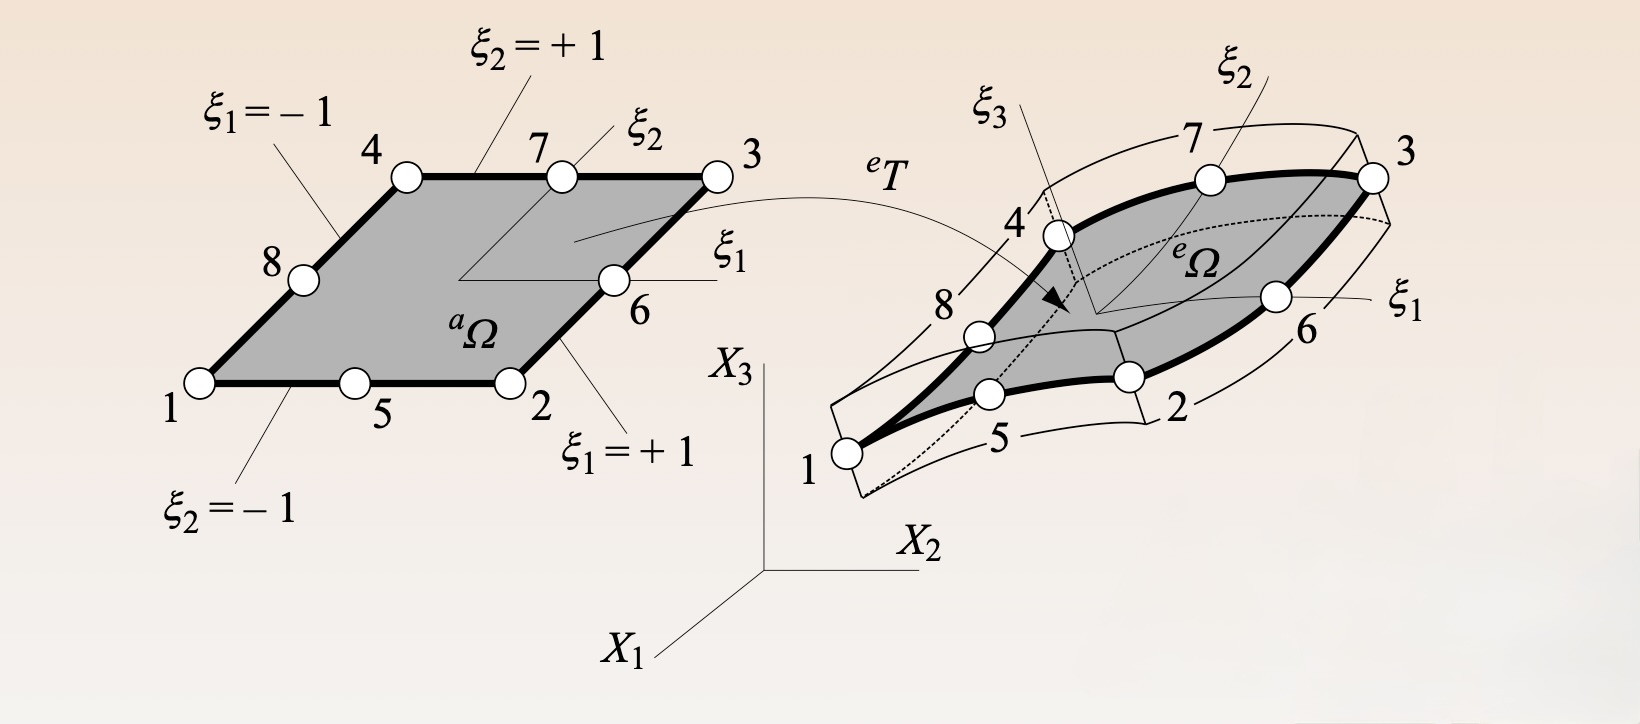
\includegraphics[height=5.5cm]{../images/shellQuad8.jpeg}
  \end{center}
\end{frame}


\begin{frame}{Example: flat shell element}
  \vspace{-0.2cm}
  \begin{center}
    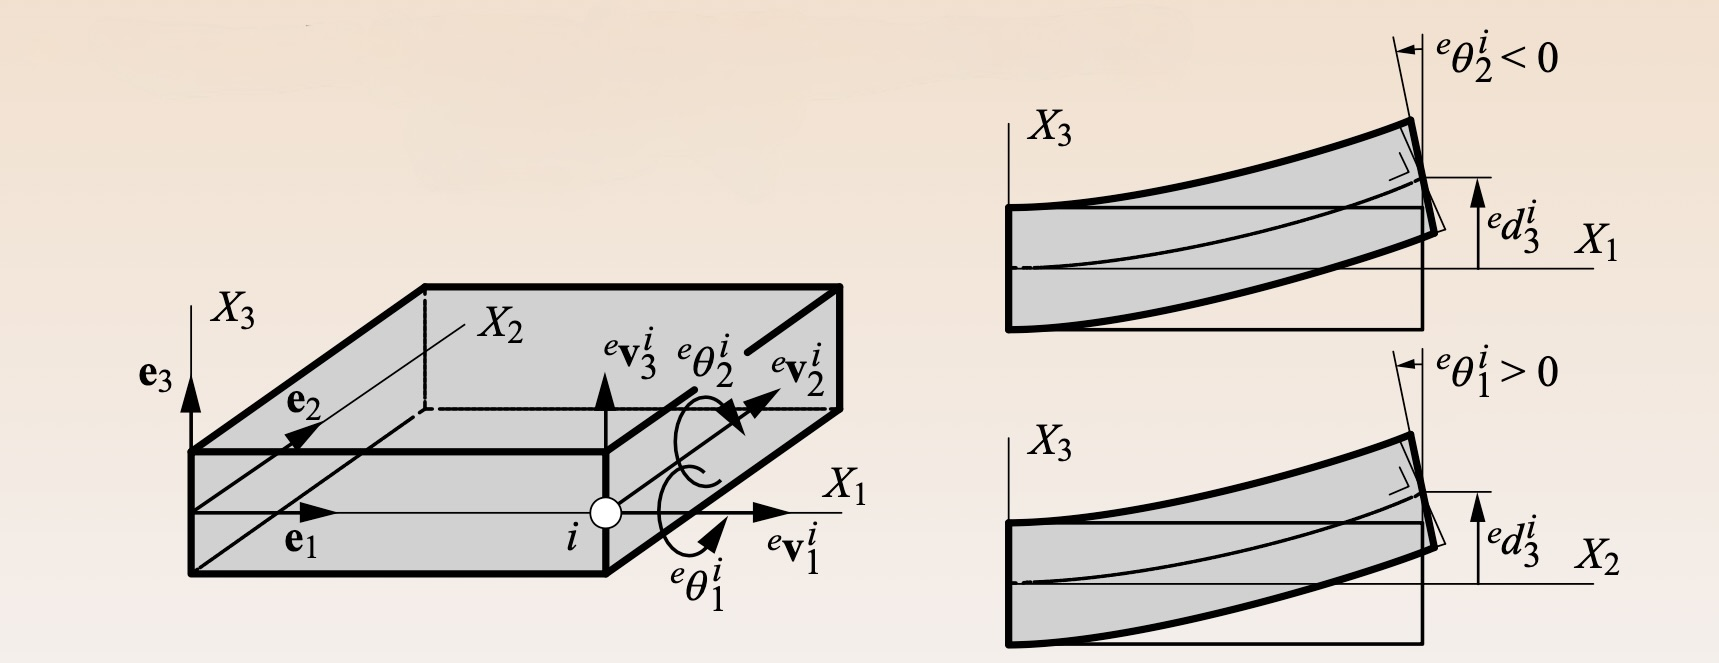
\includegraphics[height=4cm]{../images/plateBendingElem.jpeg}
  \end{center}
  \begin{align*}
    \mathbf x(\boldxi)   & =\sum_{i=1}^{{}^ep}{}^ah_i(\xi_1,\xi_2)\left(\begin{bmatrix}{}^e{x}^i \\ {}^e{y}^i  \\ 0 \end{bmatrix}
    +\frac{1}{2}\xi_3{}^e t_3^i \begin{bmatrix}0 \\ 0 \\ 1\end{bmatrix}\right)                                                                                                                                                                                                       \\
    \mathbf u^h(\boldxi) & =\sum_{i=1}^{{}^ep}{}^ah_i(\xi_1,\xi_2)\left(\begin{bmatrix}0 \\ 0 \\ {}^ed_3^i\end{bmatrix}+\frac{1}{2}\xi_3{}^e t_3^i\left(-{}^e\theta_1^i\begin{bmatrix}0 \\ 1 \\ 0\end{bmatrix}+{}^e\theta_2^i{}\begin{bmatrix}1 \\ 0 \\ 0\end{bmatrix}\right)\right)
  \end{align*}
\end{frame}

\begin{frame}{Limitation of shells with 5 degrees of freedom per node}
  Cross-section of a structure discretized with shell elements with 5 DOFs per node.
  \begin{columns}
    \begin{column}{0.33\textwidth}
      \begin{center}
        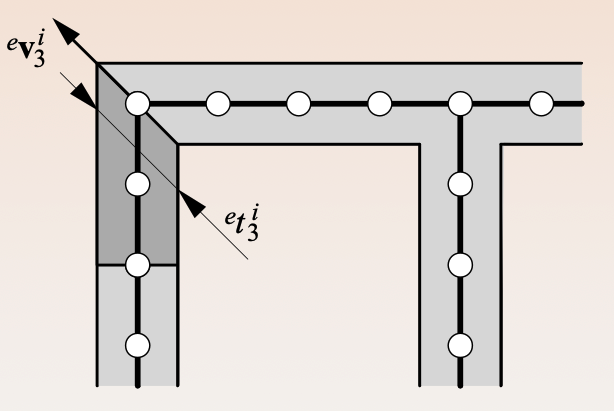
\includegraphics[height=3cm]{../images/Shell5dofs1.png}
      \end{center}
    \end{column}
    \begin{column}{0.33\textwidth}
      \begin{center}
        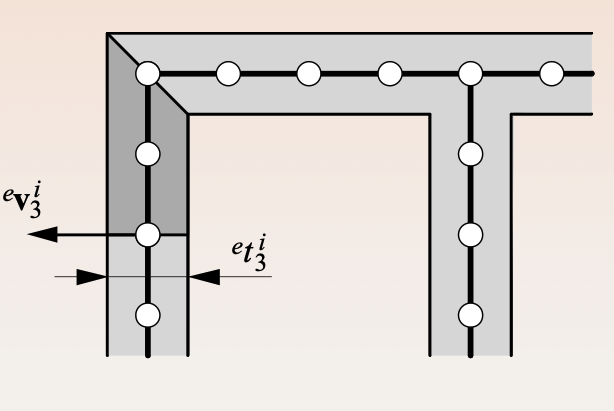
\includegraphics[height=3cm]{../images/Shell5dofs2.png}
      \end{center}
    \end{column}
    \begin{column}{0.33\textwidth}
      \begin{center}
        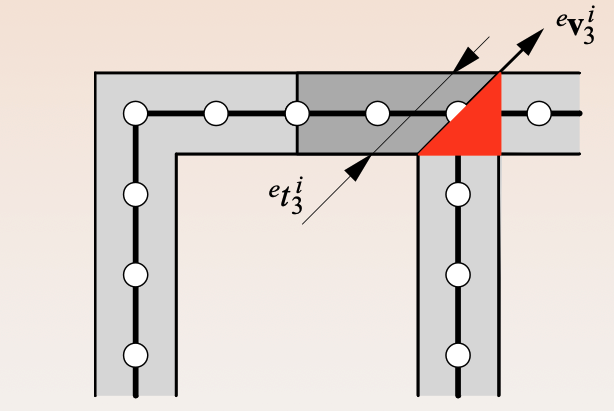
\includegraphics[height=3cm]{../images/Shell5dofs3.png}
      \end{center}
    \end{column}
  \end{columns}
  \vspace{0.3cm}
  \begin{itemize}
    \item To overcome this limitation, we need shell elements with 6 DOFs per node: 3 displacements and 3 rotations, all defined with respect to the global axis.
    \item This eliminates the need to define a local normal vector allowing for more complex geometries.
  \end{itemize}
\end{frame}

\section{Example: modal analysis of simply supported thin shell}

\begin{frame}{Simply supported isotropic thin shell}
  Discretization with $4$ bilinear quadrilateral shell elements ($4$ nodes each).

  \begin{columns}
    \column{0.45\textwidth}
    \begin{center}
      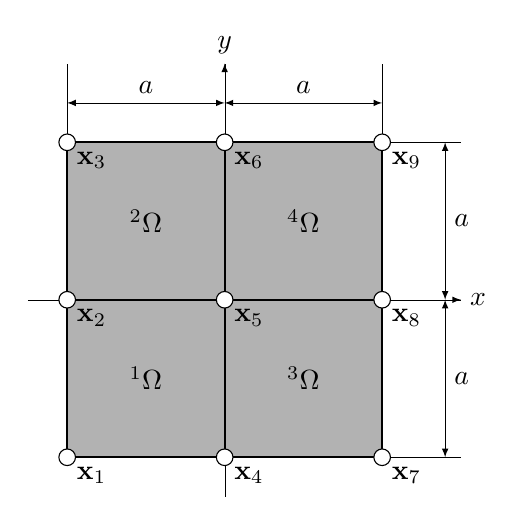
\begin{tikzpicture}[scale=1]
        \def\a{4}
        \def\b{4}
        % Draw the rectangle
        \filldraw[fill=gray!60, draw=black,thick] (0,0) rectangle (\a,\b);
        % Draw the elements  
        \draw[thick] (\a/2,0) -- (\a/2,\b);
        \draw[thick] (0,\b/2) -- (\a,\b/2);
        \node at (\a/4,\b/4) {${}^1\Omega$};
        \node at (\a/4,3*\b/4) {${}^2\Omega$};
        \node at (3*\a/4,\b/4) {${}^3\Omega$};
        \node at (3*\a/4,3*\b/4) {${}^4\Omega$};
        %axis
        \draw[-latex,ultra thin] (-0.5,\b/2) -- (\a+1,\b/2) node[right]{$x$};
        \draw[-latex, ultra thin] (\a/2,-0.5) -- (\a/2,\b+1)node[above]{$y$};
        % length
        \draw[latex-latex, ultra thin]  (0,\b+0.5)  to node[midway,above] {$a$}(\a/2,\b+0.5) ;
        \draw[latex-latex, ultra thin]  (\a/2,\b+0.5)  to node[midway,above] {$a$}(\a,\b+0.5) ;
        \draw[ultra thin] (\a/2,0) --(\a/2, \b+1);
        \draw[ultra thin] (\a,0) --(\a, \b+1) ;
        \draw[ultra thin] (0,\b/2) --(\a+1, \b/2);
        \draw[ultra thin] (0,\b) --(\a+1, \b);
        \draw[ultra thin] (\a,0) -- (\a+1,0);
        \draw[ultra thin] (0,\b) -- (0,\b+1);
        \draw[latex-latex, ultra thin]  (\a+0.8,\b/2)  to node[midway,right] {$a$}(\a+0.8,0) ;
        \draw[latex-latex, ultra thin]  (\a+0.8,\b)  to node[midway,right] {$a$}(\a+0.8,\b/2) ;
        % Nodes 
        \draw[fill=white, draw=black]  (0,0) node[below right]{$\mathbf x_1$} circle (3pt);
        \draw[fill=white, draw=black]  (0,\b/2) node[below right]{$\mathbf x_2$} circle (3pt);
        \draw[fill=white, draw=black]  (0,\b) node[below right]{$\mathbf x_3$} circle (3pt);
        \draw[fill=white, draw=black]  (\a/2,0) node[below right]{$\mathbf x_4$} circle (3pt);
        \draw[fill=white, draw=black]  (\a/2,\b/2) node[below right]{$\mathbf x_5$} circle (3pt);
        \draw[fill=white, draw=black]  (\a/2,\b) node[below right]{$\mathbf x_6$} circle (3pt);
        \draw[fill=white, draw=black]  (\a,0) node[below right]{$\mathbf x_7$} circle (3pt);
        \draw[fill=white, draw=black]  (\a,\b/2) node[below right]{$\mathbf x_8$} circle (3pt);
        \draw[fill=white, draw=black]  (\a,\b) node[below right]{$\mathbf x_9$} circle (3pt);
      \end{tikzpicture}
    \end{center}

    \column{0.5\textwidth}
    {\begin{itemize}\setlength\itemsep{0.05em}
        \item $2a$ length
        \item $2a$ height
        \item $t$ thickness
        \item $E$ Young's modulus
        \item $\nu$ Poisson's ratio
        \item $k$ shear correction factor
        \item $\rho$ material density
      \end{itemize}}
    \begin{block}{}
      \textbf{Objective:} determine the first natural frequency of the flat shell and compare it with the exact one.
    \end{block}
  \end{columns}
\end{frame}

\begin{frame}{Approximate displacements for flat shell elements}
  \begin{itemize}
    \item 5 DOFs per node ($i=1,\dots,9$): $${}^e{\mathbf q}^i=[{}^e{d}^i_1, {}^e{d}^i_2, {}^e{d}^i_3,\ {}^e{\theta}^i_1,\ {}^e{\theta}^i_2]$$
    \item Local vectors are oriented along the principal axes of the shell:
          $$ {}^e\mathbf v^i_1=[1,0,0]^T,  \qquad {}^e\mathbf v^i_2=[0,1,0]^T, \qquad {}^e\mathbf v^i_3=[0,0,1]^T$$
    \item Local shape functions matrices:
          $${}^a\mathbf H_i=
            \begin{bmatrix}
              {}^a h_i & 0        & 0        & 0                                & \dfrac{1}{2}\xi_3 t \, {}^a h_i \\
              0        & {}^a h_i & 0        & -\dfrac{1}{2}\xi_3 t \, {}^a h_i & 0                               \\
              0        & 0        & {}^a h_i & 0                                & 0                               \\
            \end{bmatrix}\qquad (i = 1, 2, 3, 4)
          $$
  \end{itemize}
\end{frame}

\begin{frame}{Coordinate transformation for ${}^1\Omega$}
  \begin{itemize}
    \item Bilinear base functions for quadrilateral shell element:
          \begin{align*}
            {}^ah_1(\xi_1,\xi_2) & =(1-\xi_1)(1-\xi_2)/4 \\
            {}^ah_2(\xi_1,\xi_2) & =(1+\xi_1)(1-\xi_2)/4 \\
            {}^ah_3(\xi_1,\xi_2) & =(1+\xi_1)(1+\xi_2)/4 \\
            {}^ah_4(\xi_1,\xi_2) & =(1-\xi_1)(1+\xi_2)/4
          \end{align*}
    \item Coordinates ${}^1\tilde{\mathbf x}=[[0,0,0],[a,0,0], [a,a,0], [0,a,0]]$
          \begin{align*}
            {}^1T: \mathbf x(\boldxi) & =\sum_{i=1}^{4}{}^ah_i(\xi_1,\xi_2)\left({}^e\tilde{\mathbf x}^i+\frac{1}{2}\xi_3{}^e t_3^i {}^e\mathbf v_3^i\right)=\left[a\frac{1+\xi_1}{2},\ a\frac{1+\xi_2}{2}, t\frac{\xi_3}{2}\right]^T
          \end{align*}
    \item Jacobian matrix ${}^1J=\text{diag}(a/2,\ a/2,\ t/2)$ and determinant ${}^1j=a^2t/8$.
  \end{itemize}
\end{frame}

\begin{frame}{Local mass matrices}
  \begin{align*}
    {}^1\mathbf M_{ij} & =\frac{\rho a^2t}{8}\int_{-1}^1\int_{-1}^1\int_{-1}^1 {}^a\mathbf H_i^T {}^a\mathbf H_j\, d\xi_1d\xi_2d\xi_3                                                                                        \\
                       & =\frac{\rho a^2t}{4}\int_{-1}^1\int_{-1}^1\begin{bmatrix}
                                                                     {}^ah_i{}^ah_j & 0              & 0 & 0                    & 0                    \\
                                                                     0              & {}^ah_i{}^ah_j & 0 & 0                    & 0                    \\ 0 & 0 & {}^ah_i{}^ah_j & 0                    & 0                    \\
                                                                     0              & 0              & 0 & t^2{}^ah_i{}^ah_j/12 & 0                    \\
                                                                     0              & 0              & 0 & 0                    & t^2{}^ah_i{}^ah_j/12 \\
                                                                   \end{bmatrix}d\xi_1d\xi_2
  \end{align*}
  Local mass matrix for ${}^1\Omega$ via exact integration:
  $${}^1\mathbf M= \begin{bmatrix}
      {}^1\mathbf M_{11} & {}^1\mathbf M_{12} & {}^1\mathbf M_{13} & {}^1\mathbf M_{14} \\
                         & {}^1\mathbf M_{22} & {}^1\mathbf M_{23} & {}^1\mathbf M_{24} \\
                         &                    & {}^1\mathbf M_{33} & {}^1\mathbf M_{34} \\
      sym.               &                    &                    & {}^1\mathbf M_{44} \\
    \end{bmatrix}$$
\end{frame}

\begin{frame}{Local deformation matrices}
  \small\vspace{-0.3cm}
  \begin{align*}
    {}^1\mathbf B_i & =\nabla {}^a\mathbf H_i = \begin{bmatrix}
                                                  \partial_{x_1} & 0              & 0              \\
                                                  0              & \partial_{x_2} & 0              \\
                                                  0              & 0              & \partial_{x_3} \\
                                                  0              & \partial_{x_3} & \partial_{x_2} \\
                                                  \partial_{x_3} & 0              & \partial_{x_1} \\
                                                  \partial_{x_2} & \partial_{x_1} & 0
                                                \end{bmatrix}\begin{bmatrix}
                                                               {}^a h_i & 0        & 0        & 0                                & \dfrac{1}{2}\xi_3 t \, {}^a h_i \\
                                                               0        & {}^a h_i & 0        & -\dfrac{1}{2}\xi_3 t \, {}^a h_i & 0                               \\
                                                               0        & 0        & {}^a h_i & 0                                & 0                               \\\end{bmatrix}                                                                           \\[1em]
                    & =\begin{bmatrix}
                         \frac{2}{a} \, \partial_{\xi_1}{}^a h_i & 0                                       & 0                                       & 0                                             & \frac{t}{a}\xi_3 \, \partial_{\xi_1}{}^a h_i \\[0.4em]
                         0                                       & \frac{2}{a} \, \partial_{\xi_2}{}^a h_i & 0                                       & -\frac{t}{a}\xi_3 \, \partial_{\xi_2}{}^a h_i & 0                                            \\[0.4em]
                         0                                       & 0                                       & \frac{2}{t} \, \partial_{\xi_3}{}^a h_i & 0                                             & 0                                            \\[0.4em]
                         0                                       & \frac{2}{t} \, \partial_{\xi_3}{}^a h_i & \frac{2}{a} \, \partial_{\xi_2}{}^a h_i & -{}^a h_i                                     & 0                                            \\[0.4em]
                         \frac{2}{t} \, \partial_{\xi_3}{}^a h_i & 0                                       & \frac{2}{a} \, \partial_{\xi_1}{}^a h_i & 0                                             & {}^a h_i                                     \\[0.4em]
                         \frac{2}{a} \, \partial_{\xi_2}{}^a h_i & \frac{2}{a} \, \partial_{\xi_1}{}^a h_i & 0                                       & -\frac{t}{a}\xi_3 \, \partial_{\xi_1}{}^a h_i & \frac{t}{a}\xi_3 \, \partial_{\xi_2}{}^a h_i \\
                       \end{bmatrix}
  \end{align*}
\end{frame}


\begin{frame}{Local stiffness matrices}
  $${}^1\mathbf K_{ij}=\frac{a^2t}{8}\int_{-1}^1\int_{-1}^1\int_{-1}^1{}^1\mathbf B_i^T\overline{\mathbf C} {}^1\mathbf B_j d\xi_1d\xi_2d\xi_3 $$
  Local stiffness matrix for ${}^1\Omega$ via exact integration
  $${}^1\mathbf K= \begin{bmatrix}
      {}^1\mathbf K_{11} & {}^1\mathbf K_{12} & {}^1\mathbf K_{13} & {}^1\mathbf K_{14} \\
                         & {}^1\mathbf K_{22} & {}^1\mathbf K_{23} & {}^1\mathbf M_{24} \\
                         &                    & {}^1\mathbf K_{33} & {}^1\mathbf K_{34} \\
      sym.               &                    &                    & {}^1\mathbf K_{44} \\
    \end{bmatrix}$$
\end{frame}

\begin{frame}{Assembly and boundary conditions}
  \vspace{-0.2cm}\begin{itemize}
    \item Since ${}^e J={}^1 J$ and thus ${}^e j={}^1 j$ for every $e=2,3,4$, we have
          $${}^e\mathbf K={}^1\mathbf K\qquad\text{and}\qquad {}^e\mathbf M={}^1\mathbf M$$
    \item The assembly of the global stiffness $\mathbf K$ ($45\times 45$) and mass matrices $\mathbf M$ ($45\times 45$) can be performed using the connectivity table:
          \[
            \begin{array}{c|cccc}
              ^e\Omega & ^1\Omega & ^2\Omega & ^3\Omega & ^4\Omega \\
              \hline
              1        & 1        & 2        & 4        & 5        \\
              2        & 4        & 5        & 7        & 8        \\
              3        & 5        & 6        & 8        & 9        \\
              4        & 2        & 3        & 5        & 6        \\
            \end{array}
          \]
    \item The following 36 DOFs are constrained due the the fact that the shell is simply supported along its perimeter:
          \begin{multicols}{4}
            $d_1^1,\ d_2^1,\ d_3^1,\ \theta_1^1,\ \theta_2^1$
            $d_1^3,\ d_2^3,\ d_3^3,\ \theta_1^3,\ \theta_2^3$
            $d_1^7,\ d_2^7,\ d_3^7,\ \theta_1^7,\ \theta_2^7$
            $d_1^9,\ d_2^9,\ d_3^9,\ \theta_1^9,\ \theta_2^9$
          \end{multicols}
          \begin{multicols}{4}
            $d_1^2,\ d_2^2,\ d_3^2,\ \theta_1^2$

            $d_1^4,\ d_2^4,\ d_3^4,\ \theta_2^4$

            $d_1^6,\ d_2^6,\ d_3^6,\ \theta_2^6$

            $d_1^8,\ d_2^8,\ d_3^8,\ \theta_1^8,$
          \end{multicols}
  \end{itemize}
\end{frame}

\begin{frame}{Modal analysis}
  \begin{itemize}
    \item The semi-discrete weak form is a system of $45-36=9$ differential equations for the 9 free DOFs: $d_3^5,\ \theta_1^5,\ \theta_2^5$, and $\theta_2^2,\ \theta_1^4,\ \theta_1^6,\ \theta_2^8$
          $$\mathbf K\mathbf q(t)+\mathbf M\ddot{\mathbf q}(t)=\mathbf 0$$
    \item The first fundamental frequency $\omega_1=\sqrt{\lambda_1}$ (in rad/s) can be computed solving the generalized eigenvalue problem: $\left(\mathbf K+\lambda\mathbf M\right)\mathbf p=\mathbf 0$.
    \item Assuming a thin plate $t/2a=0.01$ and a shear coefficient $k=5/6$ we obtain
          $$\omega_1^{approx}=0.6620\sqrt{E/(1-\nu^2)\rho a}$$
    \item From the analytical solution we obtain
          $$\omega_1^{exact}=0.0285\sqrt{E/(1-\nu^2)\rho a}$$
    \item Exact integration of transverse shear terms in the stiffness matrix $\mathbf K$ leads to \emph{element locking}.
  \end{itemize}
\end{frame}

\begin{frame}{Selective integration}
  \begin{itemize}
    \item Separate the transverse shear contributions terms ${}^e\mathbf B_i^\tau$ in the deformation matrix:
          $${}^e\mathbf B_i={}^e\mathbf B_i^\sigma+{}^e\mathbf B_i^\tau$$
    \item Split the stiffness matrix into flexural stiffness ${}^e\mathbf K^\sigma_{ij}$ and transverse shear stiffness ${}^e\mathbf K^\tau_{ij}$:
          $${}^e\mathbf K_{ij}={}^e\mathbf K^\sigma_{ij}+{}^e\mathbf K^\tau_{ij}=\int_\Omega{}^e\mathbf B_i^\sigma\overline{\mathbf C}{}^e\mathbf B_j^\sigma\, d\Omega +\int_\Omega{}^e\mathbf B_i^\tau\overline{\mathbf C}{}^e\mathbf B_j^\tau\, d\Omega$$
    \item Perform a \textbf{selective integration}: exact integration of bending contributions ${}^e\mathbf K^\sigma_{ij}$ and reduced integration (a single Gauss point located at the center of the element) for shear contributions ${}^e\mathbf K^\tau_{ij}$.
  \end{itemize}
\end{frame}

\begin{frame}{Error estimates}
  Assuming a thin squared plate $t/2a=0.01$ and a shear coefficient $k=5/6$ with selective integration we obtain:
  $$\omega_1=0.0383\sqrt{E/(1-\nu^2)\rho a}\qquad (\text{Rel. error}\approx 34\%)$$
  \begin{center}
    \begin{tabular}{ccc|c}
      \hline
      Meshing     & Integration & Elements    & Rel. error  \\
      \hline
      $2\times 2$ & Exact       & bilinear    & $>20'000\%$ \\
      $2\times 2$ & Selective   & bilinear    & $34\%$      \\
      $4\times 4$ & Selective   & bilinear    & $7.2\%$     \\
      $1\times 1$ & Selective   & biquadratic & $6.2\%$     \\
      $2\times 2$ & Selective   & biquadratic & $1.0\%$     \\
      \hline
    \end{tabular}
  \end{center}
\end{frame}

\end{document}